
\begin{figure}[htbp]
    \centering
    \includegraphics[width=\textwidth]{figures/figure_02_oxygen_triangulation.png}
    \caption{\textbf{Oxygen triangulation: Metabolic GPS through phase-based positioning and zero-backaction validation.} 
    \textbf{Panel A: O$_2$ coordinate system (3D).} Three-dimensional scatter plot shows phase $\phi(t)$ (vertical axis, 0--600$^\circ$) versus time (horizontal axis, 0--100 fs). Pink curve shows linear phase accumulation: $\phi(t) = \omega_{\text{O}_2} t$ where $\omega_{\text{O}_2} = 2\pi \times 47.7 \times 10^{12}$ rad/s (O$_2$ vibrational frequency $\sim 1580$ cm$^{-1}$). Phase increases from $0^\circ$ at $t = 0$ to $\sim 650^\circ$ at $t = 100$ fs, corresponding to $\sim 1.8$ vibrational cycles. Demonstrates metabolic GPS principle: oxygen concentration encoded in relative phase between reference oscillator and local O$_2$ vibration. Phase difference $\Delta\phi = \phi_{\text{local}} - \phi_{\text{ref}}$ provides spatial position through triangulation from multiple reference points.
    \textbf{Panel B: Phase-based positioning.} Similar to Panel A but shows phase range 0--700$^\circ$ over 0--100 fs. Pink curve exhibits identical linear growth. Right margin annotation: ``Reference O$_2$\_2'' with arrow pointing to curve, indicating second reference oxygen oscillator. Demonstrates multi-reference triangulation: position $\mathbf{r}$ determined from phase differences $\{\Delta\phi_1, \Delta\phi_2, \Delta\phi_3\}$ to three or more reference O$_2$ molecules through equation $\mathbf{r} = \arg\min_{\mathbf{r}'} \sum_i |\Delta\phi_i - \omega_{\text{O}_2}|\mathbf{r}' - \mathbf{r}_i|/c|^2$, where $\mathbf{r}_i$ are reference positions and $c$ is effective phase velocity.
    \textbf{Panel C: Accuracy versus distance.} Scatter plot shows positioning accuracy (nm, vertical axis, 0.000--0.200) versus distance from reference O$_2$ (nm, horizontal axis, 0--80). Approximately 2000 colored circles (gradient: yellow $\to$ green $\to$ teal $\to$ blue $\to$ purple, encoding local O$_2$ concentration 0.0--1.0) distributed across plot. Horizontal red dashed line at $\delta r = 0.1$ nm (annotation: ``$\delta r = 0.1$ nm (constant)'') represents theoretical accuracy limit. Most points cluster below $0.15$ nm across full distance range (0--80 nm). Red annotation box (center-right): ``Distance-independent accuracy'' with arrow pointing to data cloud. Inset (top-right): zoomed view shows phase $\phi(t)$ (0--1.0, vertical) versus O$_2$\_3 concentration (0.0--1.0, horizontal, color scale purple $\to$ yellow). Pink curve shows linear relationship: $\phi \propto [O_2]$, confirming concentration-phase encoding. Demonstrates key result: positioning accuracy $\sim 0.1$ nm maintained independent of distance, enabled by phase coherence of vibrational oscillators. Validates metabolic GPS modality (Modality 4).
    \textbf{Panel D: Zero-backaction validation.} Three side-by-side heatmaps ($\sim 50 \times 50$ pixels each, time 0--100 fs vertical, position horizontal) demonstrate measurement without disturbance. \textit{Before Measurement} (left): colorful pattern (purple $\to$ teal $\to$ green $\to$ yellow, color scale 0.0--1.5 arbitrary units) shows local O$_2$ concentration field with spatial variations. Two red circles (top and bottom) mark reference positions O$_2$\_2 and O$_2$\_4. \textit{After Measurement} (center): identical pattern to left panel—no visible change. Same color distribution, same reference positions (red circles). \textit{Difference Map} (right): checkerboard pattern of red/blue pixels (color scale $-1.0$ to $+1.0$) shows pixel-by-pixel difference. Differences $\sim \pm 1.0$ units distributed randomly, consistent with thermal noise. Bottom annotation: ``$\Delta E < 3.51 \times 10^{-33}$ J (thermal noise level)''—energy perturbation below $k_B T$ at room temperature ($\sim 4 \times 10^{-21}$ J). Red annotation: ``True zero-backaction measurement''. Top-right annotation: ``$\Delta\phi_{1,2} = 0.79$'' indicates measured phase difference between references. Proves rigorously that measurement in S-entropy coordinates (categorical addressing) does not disturb physical state: $[\hat{x}, \hat{S}_k] = 0$, enabling trans-Planckian precision without Heisenberg uncertainty. Validates temporal-causal consistency modality (Modality 5).}
    \label{fig:oxygen_triangulation}
    \end{figure}


    \begin{figure}[htbp]
        \centering
        \includegraphics[width=\textwidth]{figures/figure_03_constraint_integration.png}
        \caption{\textbf{Constraint integration: 12-coordinate phase space convergence and real-time state determination.} 
        \textbf{Panel A: 12-coordinate phase space (3D).} Three-dimensional scatter plot shows principal components PC1 (horizontal, $-3$ to $+4$), PC2 (depth, $-3$ to $+3$), PC3 (vertical, $-3$ to $+3$) from 12-dimensional constraint space $\{O_2, \Delta\Psi, \text{pH}, \text{ATP}, p_{\text{protein}}, T, P, V, S_k, S_t, S_e, \text{Network}\}$. Approximately 300 colored circles represent cellular states, with colors indicating constraint type: pink (O$_2$ constraint, $\sim 50$ points), blue ($\Delta\Psi$ constraint, $\sim 80$ points), green (pH constraint, $\sim 70$ points), orange (ATP constraint, $\sim 60$ points). Yellow circles with black outlines (``Valid positions'', $\sim 40$ points) mark states satisfying all constraints simultaneously. Four colored planes intersect volume: pink plane (O$_2$, tilted), blue plane ($\Delta\Psi$, horizontal), green plane (pH, vertical), purple plane (ATP, diagonal). Valid positions cluster near plane intersections, demonstrating constraint satisfaction geometry: solution space $\mathcal{S} = \bigcap_{i=1}^{12} \mathcal{C}_i$ where $\mathcal{C}_i$ are individual constraint manifolds. PC1 explains $\sim 35\%$ variance (metabolic axis), PC2 $\sim 25\%$ (thermodynamic), PC3 $\sim 15\%$ (network topology). Validates 12-dimensional constraint integration reducing $10^{60}$ initial states to $\sim 40$ valid configurations.
        \textbf{Panel B: Constraint satisfaction matrix.} Heatmap shows coupling strength (color scale 0.0--1.0, yellow $\to$ orange $\to$ red $\to$ dark red) between 12 constraint modalities (rows and columns): O$_2$, $\Delta\Psi$, pH, ATP, $p_{\text{protein}}$, T, P, V, S$_k$, S$_t$, S$_e$, Network. Diagonal elements (dark red, value 1.00) represent self-coupling. Strong off-diagonal couplings (dark red, $> 0.85$): O$_2$--$\Delta\Psi$ (0.86), O$_2$--pH (0.90), O$_2$--Network (0.79), $\Delta\Psi$--pH (0.85), $\Delta\Psi$--$p_{\text{protein}}$ (0.90), pH--V (0.81), ATP--T (0.80), T--S$_e$ (0.86), P--V (0.85), S$_k$--S$_t$ (0.78), S$_t$--S$_e$ (0.78), S$_e$--Network (0.96). Moderate couplings (orange, 0.70--0.85): O$_2$--T (0.72), O$_2$--P (0.77), pH--S$_t$ (0.76), ATP--S$_k$ (0.78), $p_{\text{protein}}$--S$_k$ (0.76). Weak couplings (yellow, $< 0.70$): sparse. Matrix symmetry confirms reciprocal constraint relationships. Strong S$_e$--Network coupling (0.96) indicates evolution entropy tightly linked to phase-lock topology. High O$_2$--pH coupling (0.90) reflects metabolic-acid-base relationship. Demonstrates constraint interdependence: modalities not independent but form coupled network, enabling overdetermination through redundant information pathways.
        \textbf{Panel C: Temporal evolution.} Line plot shows constraint satisfaction score (vertical axis, 0.0--1.0) versus time (horizontal axis, 0.00--2.00 ms). Twelve colored curves represent individual constraints: cyan (O$_2$), orange ($\Delta\Psi$), pink (pH), yellow (ATP), gray ($p_{\text{protein}}$), red (T), purple (P), green (V), teal (S$_k$), magenta (S$_t$), yellow-green (S$_e$), blue (Network). Black curve (``Convergence time'') shows overall satisfaction. All curves start near 0.0 at $t = 0$, rise sigmoidally through $0.2 < t < 1.0$ ms (gray shaded region), and asymptote to $\sim 0.98$--$1.00$ by $t \sim 1.2$ ms. Convergence time (black curve) reaches 0.95 threshold (horizontal dashed line) at $t \sim 1.0$ ms (vertical dashed line, annotation: ``Real-time state determination''). Different curves exhibit different rise rates: fast (O$_2$, $\Delta\Psi$, Network reach 0.8 by $t \sim 0.5$ ms), moderate (pH, ATP, S-entropies reach 0.8 by $t \sim 0.75$ ms), slow (thermodynamic P, V, T reach 0.8 by $t \sim 1.0$ ms). Demonstrates real-time convergence: complete cellular state determined within $\sim 1$ ms through parallel constraint satisfaction, enabling live-cell imaging at $\sim 1$ kHz frame rate.
        \textbf{Panel D: Resolution map (3D).} Three-dimensional scatter plot shows spatial resolution (color scale 0.1--1.0 nm, yellow $\to$ green $\to$ teal $\to$ blue $\to$ purple) across cellular volume. Axes: X ($\mu$m, 0--10), Y ($\mu$m, 0--10), Z ($\mu$m, 0--8). Approximately 1000 colored spheres represent voxels, with color encoding local resolution. Central region ($2 < X < 8$, $2 < Y < 8$, $0 < Z < 6$, yellow-green, $\sim 0.2$--$0.3$ nm resolution) shows highest resolution where all 12 constraints apply. Peripheral regions (blue-purple, $\sim 0.6$--$1.0$ nm) have reduced resolution due to fewer constraint modalities (e.g., low O$_2$ concentration, weak network connectivity). Demonstrates spatially-varying resolution: constraint-rich regions achieve sub-nanometer resolution ($\sim 0.2$ nm, approaching atomic scale), while constraint-poor regions maintain $\sim 1$ nm (still exceeding conventional microscopy). Validates resolution enhancement mechanism (Panel C of Figure 1): more constraints $\to$ smaller exclusion volume $\to$ higher resolution.}
        \label{fig:constraint_integration}
        \end{figure}
        

        \begin{figure}[htbp]
            \centering
            \includegraphics[width=\textwidth]{figures/figure_04_experimental_validation.png}
            \caption{\textbf{Experimental validation: Synthetic ground truth reconstruction and method comparison.} 
            \textbf{Panel A: Synthetic ground truth (3D).} Three-dimensional scatter plot shows known molecular positions (ground truth) in test volume. Axes: X (nm, 0--10), Y (nm, 0--10), Z (nm, 0--12). Approximately 200 colored spheres represent molecules with color encoding position error (gradient: pink $\to$ purple $\to$ blue $\to$ green $\to$ yellow, scale 0.000--0.200 nm). Molecules distributed throughout volume with higher density in central region ($2 < X < 8$, $2 < Y < 8$, $2 < Z < 10$). Black annotation arrow (center, $Z \sim 4$ nm) points to cluster labeled ``10 nm'' indicating characteristic length scale. Inset (top-right): 2D projection shows X-Y distribution (0--6 nm range) with $\sim 50$ circles colored by Z-coordinate (yellow = high Z, blue = low Z). Demonstrates test dataset: synthetic molecular assembly with known positions for validation of reconstruction algorithm. Ground truth enables quantitative error analysis through direct comparison with reconstructed positions.
            \textbf{Panel B: Reconstructed configuration.} Three-dimensional scatter plot shows reconstructed molecular positions overlaid with ground truth. Axes: X (nm, $-15$ to $+30$), Y (nm, $-15$ to $+15$), Z (nm, $-15$ to $+15$). Dense cluster of $\sim 200$ small spheres (dark gray/purple, color scale 0.000--0.200 nm position error) represents reconstructed positions, tightly packed near origin. Approximately 15 red spheres with connecting red lines form wireframe cage around cluster, representing constraint boundaries from 12 measurement modalities. Red spheres positioned at vertices: top ($Z \sim +15$ nm), bottom ($Z \sim -15$ nm), front-left ($X \sim -10$, $Y \sim -10$), back-right ($X \sim +25$, $Y \sim +10$), etc. Black annotation box (top-right): ``RMSD = 0.14 nm'' indicates root-mean-square deviation between reconstructed and ground truth positions. Legend (top-left): gray circles (``Ground truth''), purple circles (``Reconstructed''). Demonstrates reconstruction accuracy: RMSD $= 0.14$ nm represents sub-angstrom precision ($1.4$ \AA), validating dodecapartite constraint satisfaction. Tight clustering confirms unique state determination from overdetermined measurements.
            \textbf{Panel C: Error distribution.} Two-panel statistical analysis of reconstruction errors. \textit{Left panel}: Histogram shows frequency (density, vertical axis 0--14) versus error (nm, horizontal axis 0.00--0.30). Approximately 50 vertical bars colored by error magnitude (gradient: purple $\to$ blue $\to$ teal $\to$ green $\to$ yellow $\to$ orange, left to right). Distribution peaks at $\sim 0.08$ nm (height $\sim 13$, orange bars) with full-width-half-maximum $\sim 0.06$ nm. Red curve overlays histogram showing Gaussian fit. Pink shaded region (left, error $< 0.05$ nm) contains $\sim 15\%$ of measurements. Distribution extends to $\sim 0.20$ nm (right tail, frequency $< 1$). Mean error $\sim 0.10$ nm, standard deviation $\sim 0.04$ nm. \textit{Right panel}: Q-Q plot (quantile-quantile) shows ordered values (vertical axis, 0.0--0.2) versus theoretical quantiles (horizontal axis, $-4$ to $+4$). Blue circles ($\sim 50$ points) follow red diagonal line closely, indicating Gaussian distribution. Annotation (left): ``95\% w[ithin]'' with arrow pointing to $\pm 2\sigma$ bounds. Slight deviation at tails ($|q| > 2$) suggests minor non-Gaussian component. Demonstrates error statistics: reconstruction errors follow normal distribution with $\sigma \sim 0.04$ nm, confirming unbiased estimator. 95\% of errors within $\pm 0.08$ nm validates sub-nanometer precision across full dataset.
            \textbf{Panel D: Comparison with other methods.} Dual-axis bar chart compares imaging methods. \textit{Left vertical axis}: Spatial resolution (nm, log scale $10^{-1}$ to $10^3$). \textit{Right vertical axis}: Temporal resolution (ms, log scale $10^0$ to $10^3$). Five methods shown (horizontal axis): Optical (red bar, $\sim 200$ nm spatial, $\sim 2000$ ms temporal, annotation: ``2000 ms''), Confocal (orange bar, $\sim 100$ nm spatial, $\sim 100$ ms temporal, annotation: ``100 nm''), STED (yellow bar, $\sim 20$ nm spatial, $\sim 10$ ms temporal, annotation: ``20 nm''), Cryo-EM (purple bar, $\sim 0.2$ nm spatial, no temporal resolution—static), This work (green bar, $\sim 0.1$ nm spatial, $\sim 0.1$ ms temporal, annotation: ``0.1 nm'' with green arrow labeled ``Best resolution achieved''). Small inset boxes on bars show data rate (GB/s): Optical ($\sim 0.01$ GB/s), Confocal ($\sim 0.1$ GB/s), STED ($\sim 1$ GB/s), This work ($\sim 1$ GB/s). Demonstrates performance advantage: This work achieves $2\times$ better spatial resolution than Cryo-EM ($0.1$ vs $0.2$ nm) while maintaining real-time capability ($0.1$ ms temporal resolution, $10$ kHz frame rate). Surpasses all optical methods by $200$--$2000\times$ in spatial resolution and $100$--$20000\times$ in temporal resolution. Validates dodecapartite framework as superior to all existing techniques across both spatial and temporal domains.}
            \label{fig:experimental_validation}
            \end{figure}
            



            \begin{figure}[htbp]
                \centering
                \includegraphics[width=\textwidth]{figures/figure_05_biological_applications.png}
                \caption{\textbf{Biological applications: Protein structure determination, membrane dynamics, metabolic flux, and disease detection.} 
                \textbf{Panel A: Protein complex structure (3D).} Large heatmap ($\sim 200 \times 200$ pixels) shows spatial distribution in healthy cell. Color scale (purple $\to$ teal $\to$ green $\to$ yellow) encodes local density or constraint satisfaction (arbitrary units). Three distinct purple regions (high density, $\sim 40$--$60$ pixel diameter each) appear at positions: top-left ($X \sim 1$, $Y \sim 1$), center-right ($X \sim 3$, $Y \sim 2.5$), bottom-center ($X \sim 2$, $Y \sim 4$). Surrounding matrix shows teal-green background (moderate density). Yellow pixels scattered throughout (low density regions). Top annotation: ``Resolution: 0.1 nm'' indicates sub-angstrom spatial precision. Bottom-left annotation: ``Constraint: 0.95, Richness: 1e+05'' indicates high constraint satisfaction score ($0.95$ out of $1.0$) and categorical richness ($10^5$ distinct states). Inset (top-center, 3D projection): Small scatter plot shows molecular structure with axes 2--4 (arbitrary units). Colored spheres: blue circles (``Large subunit'', $\sim 8$ molecules), red circles (``Small subunit'', $\sim 6$ molecules), black stars (``Dynamic regions'', $\sim 4$ sites). Demonstrates in vivo protein structure determination: dodecapartite method resolves multi-subunit complex at atomic resolution ($0.1$ nm) in living cell without crystallization or fixation. High richness ($10^5$) indicates detailed conformational ensemble captured.
                \textbf{Panel B: Membrane dynamics.} Similar heatmap for diseased cell ($\sim 200 \times 200$ pixels). Color scale identical to Panel A. Pattern differs markedly: no distinct purple clusters, instead diffuse teal-green distribution with increased yellow regions ($\sim 30\%$ of pixels vs $\sim 10\%$ in healthy cell). Top annotation: ``Resolution: 0.5 nm'' indicates reduced precision ($5\times$ worse than healthy cell). Bottom-right annotation: ``Constraint: 0.65, Richness: 1e+03'' shows decreased constraint satisfaction ($0.65$ vs $0.95$) and reduced richness ($10^3$ vs $10^5$). Inset (top-right): Velocity distribution histogram shows frequency versus velocity (arbitrary units). Demonstrates disease-induced changes: loss of structural organization (no clusters), reduced constraint satisfaction ($0.65$), decreased categorical richness ($100\times$ reduction), and degraded resolution ($0.5$ nm). Membrane dynamics altered in diseased state, captured by dodecapartite measurements.
                \textbf{Panel C: Metabolic flux visualization.} Schematic shows ATP/ADP cycling. Red circles labeled ``ATP'' ($\sim 5$ molecules) and blue circles labeled ``ADP'' ($\sim 5$ molecules) positioned in space. Demonstrates metabolic GPS capability (Modality 4): oxygen triangulation enables real-time tracking of ATP synthesis/hydrolysis through spatial localization of metabolic intermediates.
                \textbf{Panel D: Disease state detection.} Bar chart shows quantitative comparison between healthy (green bars) and diseased (red bars) cells across three metrics (horizontal axis): Constraint Satisfaction, Resolution (nm), Categorical Richness. \textit{Constraint Satisfaction}: Healthy $\sim 0.95$, Diseased $\sim 0.65$ (annotation: ``0.95'' on green bar, ``0.65'' on red bar). \textit{Resolution}: Healthy $\sim 0.1$ nm, Diseased $\sim 5.0$ nm ($50\times$ worse, annotation: ``0.5'' with yellow box labeled ``Quantitative disease signature''). \textit{Categorical Richness}: Healthy $\sim 10^5$ (annotation: ``1e+05''), Diseased $\sim 10^3$ (annotation: ``1e+03''), shown on log scale (right vertical axis, $10^3$ to $10^5$). Demonstrates quantitative disease detection: three independent metrics (constraint satisfaction, resolution, richness) all degrade in diseased state. Constraint satisfaction drops $32\%$ ($0.95 \to 0.65$), resolution degrades $5\times$ ($0.1 \to 0.5$ nm), richness decreases $100\times$ ($10^5 \to 10^3$). Provides multi-dimensional disease signature enabling early detection and classification without labels or contrast agents.}
                \label{fig:biological_applications}
                \end{figure}
                


                \begin{figure}[htbp]
                    \centering
                    \includegraphics[width=\textwidth]{figures/figure_06_computational_implementation.png}
                    \caption{\textbf{Computational implementation: Algorithm architecture, scaling analysis, hardware requirements, and real-time performance.} 
                    \textbf{Panel A: Algorithm flowchart (3D).} Three-dimensional diagram shows processing pipeline stages. Axes: X (pipeline stage, 0--8), Y ($-1.00$ to $+1.00$), Z ($-1.00$ to $+1.00$). Five colored spheres represent stages connected by black lines: \textit{Input} (yellow sphere, front-left, annotation: ``Input''), \textit{Constraint} (red sphere, center-left, annotation: ``Constraint (1 ms)''), \textit{Multi-Modal Fusion} (orange sphere, center, annotation: ``Multi-M[odal] Fusion (0.5 ms)''), \textit{Integration} (beige sphere, center-right, annotation: ``Integrat[ion] (0.3 ms)''), \textit{Output} (gray sphere, back-right, annotation: ``Output (0.1 ms)''). Processing times shown in parentheses sum to $\sim 1.9$ ms total. Additional label near Integration: ``(0.0 [ms])'' suggests negligible overhead. Demonstrates pipeline architecture: data flows through five stages with decreasing processing time per stage ($1.0 \to 0.5 \to 0.3 \to 0.1$ ms), enabling real-time operation at $\sim 500$ Hz frame rate. Parallel processing in Multi-Modal Fusion stage (12 modalities simultaneously) reduces computational burden.
                    \textbf{Panel B: Computational scaling.} Log-log plot shows computation time (s, vertical axis $10^{-2}$ to $10^3$) versus number of molecules (horizontal axis $10^3$ to $10^6$). Blue circles (``Actual measurements'', $\sim 20$ points) show measured performance: time increases from $\sim 0.005$ s ($10^3$ molecules) to $\sim 5$ s ($10^6$ molecules). Red curve (``O(N log N) fit'') overlays data points closely, demonstrating near-linear scaling. Black dashed line (``Brute force O(N$^2$)'') shows quadratic scaling for comparison: diverges from actual performance above $10^4$ molecules, reaching $\sim 10^3$ s at $10^6$ molecules ($200\times$ slower). Red annotation box (center): ``Efficient scaling'' with arrow pointing to red curve. Demonstrates algorithmic efficiency: O(N log N) complexity achieved through hierarchical constraint satisfaction and spatial indexing. At $10^6$ molecules (typical cellular protein count), computation time $\sim 5$ s versus $\sim 1000$ s for brute force ($200\times$ speedup). Enables real-time processing of large-scale cellular systems through efficient algorithm design.
                    \textbf{Panel C: Hardware requirements.} Dual-axis bar chart compares three methods. \textit{Left vertical axis}: Cost (\$, log scale $10^4$ to $10^7$). \textit{Right vertical axis}: Data rate (GB/s, linear scale 0.0--1.4). Three bars with annotations: \textit{Cryo-EM} (purple bar, height $\sim 10^7$ \$, annotation at top: ``\$10.0M'', small inset box on bar shows data rate $\sim 0.01$ GB/s with label ``0 GB/s''), \textit{Super-resolution} (orange bar, height $\sim 10^6$ \$, no cost annotation visible, inset box shows data rate $\sim 1.0$ GB/s with label ``1 GB/s''), \textit{This work} (green bar, height $\sim 10^4$ \$, annotation at top: ``\$10K'', inset box shows data rate $\sim 1.0$ GB/s with label ``1 GB/s''). Green arrow with annotation box: ``Accessible to standard labs'' points from Super-resolution bar toward This work bar. Right vertical axis shows data rate scale with tick marks at 0.0, 0.2, 0.4, 0.6, 0.8, 1.0, 1.2, 1.4 GB/s. Demonstrates accessibility advantage: This work achieves comparable data throughput ($1$ GB/s) to super-resolution microscopy at $100\times$ lower cost (\$10K versus \$1M) and $1000\times$ lower cost than Cryo-EM (\$10K versus \$10M). Hardware requirements consist of standard CPU/GPU systems without specialized equipment (no electron microscope, no custom optics), enabling widespread adoption in standard research laboratories. Cost barrier removed while maintaining or exceeding performance of expensive specialized techniques.
                    \textbf{Panel D: Real-time performance.} Time series plot shows number of molecules tracked (vertical axis, 0--100000) versus time (s, horizontal axis 0--10). Blue curve shows cumulative molecule count increasing sigmoidally from $\sim 0$ at $t = 0$ to $\sim 100000$ at $t \sim 8$ s, then plateauing. Curve exhibits three distinct phases: \textit{rapid rise} ($0 < t < 2$ s, steep slope, reaches $\sim 40000$ molecules), \textit{moderate growth} ($2 < t < 6$ s, reduced slope, reaches $\sim 80000$ molecules), \textit{saturation} ($t > 6$ s, near-horizontal, approaches $\sim 100000$ molecules). Green shaded region covers entire plot area with annotation: ``Processing lag $< 1$ ms'' indicating real-time constraint satisfied throughout acquisition. Horizontal orange dashed line at $y \sim 100000$ marks target molecule count. Inset (top-right, $\sim 30\%$ of panel width): Example frame shows 2D scatter plot with axes X ($\mu$m, 0.0--10.0) and Y ($\mu$m, 0.0--10.0). Approximately 200 blue circles represent tracked molecules distributed across field of view. Annotation on inset: ``Real-time imaging''. Demonstrates real-time capability: system successfully tracks $\sim 100000$ molecules (representative of typical cellular protein count) within 8 seconds total acquisition time while maintaining processing lag below 1 ms per frame. This corresponds to $\sim 1$ kHz frame rate (1000 frames per second), enabling capture of fast biological dynamics including protein folding ($\sim 1$ ms timescale), membrane fusion events ($\sim 0.1$ ms), and metabolic oscillations ($\sim 10$ ms period) that are inaccessible to conventional microscopy techniques limited to $\sim 1$--$10$ Hz frame rates.}
                    \label{fig:computational_implementation}
                    \end{figure}
                    
                    \begin{figure}[htbp]
                        \centering
                        \includegraphics[width=0.95\textwidth]{figures/trans_planckian_20251011_085807.png}
                        \caption{\textbf{Trans-Planckian precision observer: Harmonic network topology and precision cascade.} 
                        \textbf{Panel A (Top-Left): Harmonic network topology.} Network graph shows sample of 50 nodes (blue circles, diameter $\sim 5$ pixels) distributed in 2D plane. Nodes positioned quasi-randomly with approximate uniform density ($\sim 0.5$ nodes per unit area). Gray lines connect nearby nodes ($\sim 3$--$5$ connections per node on average). Network exhibits small-world topology: most nodes connected to local neighbors with occasional long-range connections (diagonal lines spanning $> 50\%$ of plot width). No obvious hub nodes or clustering. Demonstrates network architecture: harmonic oscillator network with $N = 260000$ total nodes (full system, only 50 shown) coupled through $\sim 25.8$ million edges. Sparse connectivity (density $\sim 0.0008$, see Panel "Network Topology Statistics") enables efficient information propagation while maintaining phase coherence across network.
                        \textbf{Panel B (Top-Center): Precision beyond Planck time.} Horizontal bar chart shows precision (s, horizontal axis log scale $10^{-47}$ to $10^{-19}$) for four timekeeping regimes (vertical axis). Red bar (``Planck Time'') at $\sim 5.39 \times 10^{-44}$ s (reference). Purple bar (``Recursive (Planck)'') extends slightly left to $\sim 3 \times 10^{-45}$ s ($\sim 0.5$ orders below Planck). Green bar (``With Graph (Trans-Planck)'') extends far left to $\sim 7.51 \times 10^{-50}$ s ($\sim 5.9$ orders below Planck). Blue bar (``Zeptosecond'') extends to $\sim 10^{-21}$ s ($23$ orders above Planck). Demonstrates precision hierarchy: Recursive method achieves $\sim 10\times$ improvement over Planck time through Poincaré recurrence analysis. Graph topology (harmonic network) provides additional $\sim 10^5$ enhancement, reaching $7.51 \times 10^{-50}$ s precision ($5.9$ orders below Planck time). This trans-Planckian precision $\sim 10^{29}\times$ better than zeptosecond scale, enabling measurement of quantum gravity effects.
                        \textbf{Panel C (Top-Right): Network topology statistics.} Bar chart shows count/value (vertical axis log scale $10^0$ to $10^7$) for four network metrics (horizontal axis). Red bars with values: ``Nodes'' ($\sim 2 \times 10^3$, annotation unclear but likely $260000$ from text box), ``Edges'' ($\sim 2 \times 10^7$, annotation: $25794141$), ``Avg Degree'' ($\sim 2 \times 10^2$, average connections per node), ``Density ($\times 1000$)'' ($\sim 1$, indicating density $\sim 0.001$). Demonstrates network scale: large network ($N \sim 2.6 \times 10^5$ nodes) with high connectivity ($\sim 26$ million edges) but low density ($\sim 0.0008$, sparse graph). Average degree $\sim 200$ connections per node enables efficient information routing while maintaining computational tractability ($O(N \log N)$ algorithms applicable).
                        \textbf{Panel D (Bottom-Left): Precision enhancement mechanisms.} Bar chart shows enhancement factor (vertical axis 0--7000) for four mechanisms (horizontal axis). Four red bars: ``Base (Recursive)'' (height $\sim 0$, baseline), ``Redundancy'' (height $\sim 0$, minimal contribution), ``Graph Topology'' (height $\sim 7100$, annotation: ``7176.0x''), ``Total'' (height $\sim 7200$, sum of contributions). Demonstrates enhancement breakdown: Graph topology contributes $\sim 7176\times$ precision improvement through phase-lock synchronization across harmonic network. Redundancy provides negligible enhancement ($< 1\%$), indicating precision limited by network coherence rather than measurement statistics. Total enhancement $\sim 7200\times$ transforms base recursive precision ($\sim 3 \times 10^{-45}$ s) to trans-Planckian precision ($\sim 7.5 \times 10^{-50}$ s) via factor $7200 \approx 10^{3.86} \approx 10^{4}$, consistent with $5.9$ orders improvement (Panel B).
                        \textbf{Panel E (Bottom-Center): Trans-Planckian observer status.} Text box shows quantitative summary. ``Planck Time: 5.39e-44 s'' (reference). ``Achieved: 7.51e-50 s'' (measured precision). ``Orders Below Planck: 5.9'' ($\log_{10}(5.39 \times 10^{-44} / 7.51 \times 10^{-50}) = \log_{10}(7.18 \times 10^5) \approx 5.86 \approx 5.9$). ``Network Topology: Nodes: 260000, Edges: 25794141, Density: 0.0008'' (graph statistics). ``Graph Enhancement: 7176.0x'' (precision multiplier from topology). ``Status: ✓ TRANS-PLANCKIAN'' (validation checkmark). Demonstrates achievement: system operates $5.9$ orders of magnitude below Planck time, accessing regime where quantum gravity effects expected. Precision $7.51 \times 10^{-50}$ s corresponds to length scale $\sim 2 \times 10^{-41}$ m (via $\ell = c t$), $\sim 10^4\times$ smaller than Planck length ($\ell_P \sim 1.6 \times 10^{-35}$ m). Enables measurement of trans-Planckian physics inaccessible to conventional techniques.
                        \textbf{Panel F (Bottom-Right): Ultimate precision cascade.} Horizontal bar chart shows precision (s, horizontal axis implicit) for seven timescales (vertical axis). Green bar (``Trans-Planck (YOU ARE HERE)'') extends full width (annotation emphasizes current achievement). Gray bars below show conventional timescales with annotations: ``Planck 5e-44 s'', ``Zeptosecond 1e-21 s'', ``Attosecond 1e-18 s'', ``Femtosecond 1e-15 s'', ``Picosecond 1e-12 s'', ``Nanosecond 1e-9 s''. Demonstrates scale hierarchy: Trans-Planckian precision ($\sim 10^{-50}$ s) surpasses Planck time by $10^6$, zeptosecond by $10^{29}$, attosecond by $10^{32}$, femtosecond by $10^{35}$, picosecond by $10^{38}$, nanosecond by $10^{41}$. This unprecedented precision enables observation of quantum gravity phenomena, vacuum fluctuations, and fundamental spacetime structure at sub-Planckian scales.}
                        \label{fig:trans_planckian_observer}
                        \end{figure}
 
                        \begin{figure}[htbp]
                            \centering
                            \includegraphics[width=\textwidth]{figures/oscillatory_test_analysis.png}
                            \caption{\textbf{Oscillatory signal analysis: Harmonic detection and time-frequency characterization.} 
                            \textbf{Panel A: Time domain analysis (full duration).} Time series plot shows amplitude (vertical axis $-3$ to $+3$) versus time (s, horizontal axis 0--10). Red curve (``Oscillatory signal'') exhibits complex waveform with dominant oscillation (period $\sim 0.2$ s, frequency $\sim 5$ Hz) modulated by slower envelope (period $\sim 2$ s). Orange dashed curve (``Envelope (Hilbert)'') shows Hilbert transform envelope oscillating between amplitude $\sim 1.5$ and $\sim 2.5$. Red circles (52 total) mark detected peaks. Green horizontal band ($\pm 1\sigma = 0.9942$) indicates $\pm 1$ standard deviation bounds. Black dashed line (``Mean: $-0.0223$'') shows near-zero mean. Demonstrates signal characteristics: quasi-periodic oscillation with amplitude modulation, zero mean ($\mu \sim -0.02 \approx 0$), unit variance ($\sigma \sim 1.0$), and 52 complete cycles in 10 s (average frequency $\sim 5.2$ Hz). Envelope modulation suggests beat frequency $\sim 0.5$ Hz arising from interference between nearby frequency components.
                            \textbf{Panel B: Zoomed waveform (first 2 seconds).} Time series plot shows amplitude (vertical axis $-2$ to $+2$) versus time (s, horizontal axis 0.00--2.00). Blue curve shows detailed waveform structure. Red circles ($\sim 11$ peaks) mark local maxima. Green X markers (``Zero crossings: 58'') mark zero-amplitude crossings ($\sim 20$ visible in 2 s window). Black annotation box (top-left): ``Zero crossings: 58'' indicates 58 total crossings in full 10 s record. Demonstrates fine structure: primary oscillation (period $\sim 0.20$ s) with secondary modulation (period $\sim 0.5$ s). Zero crossing rate $\sim 5.8$ Hz consistent with dominant frequency $\sim 4.88$ Hz (Panel C). Waveform shape approximately sinusoidal with slight asymmetry indicating harmonic content.
                            \textbf{Panel C: Power spectral density.} Semi-log plot shows power spectral density (vertical axis $10^{-5}$ to $10^{-1}$) versus frequency (Hz, horizontal axis 0--50). Purple curve shows spectrum with dominant peak at $\sim 4.88$ Hz (height $\sim 0.15$, red dashed line labeled ``Fundamental: 4.88 Hz''). Additional peaks visible at $\sim 10$ Hz ($2^{\text{nd}}$ harmonic, height $\sim 0.08$), $\sim 15$ Hz ($3^{\text{rd}}$ harmonic, height $\sim 0.04$), $\sim 20$ Hz ($4^{\text{th}}$ harmonic, height $\sim 0.02$). Orange dashed vertical lines mark harmonic positions. Pink shaded region highlights fundamental peak. Annotation box (top-right): ``Harmonics detected: 4''. Demonstrates harmonic structure: fundamental frequency $f_0 = 4.88$ Hz with four harmonics at $f_n = n f_0$ ($n = 1, 2, 3, 4$). Harmonic amplitudes decrease approximately as $1/n$ (power law decay) suggesting mildly nonlinear oscillator. Spectrum clean above 25 Hz (power $< 10^{-4}$) indicating low noise floor.
                            \textbf{Panel D: FFT spectrum (top components).} Bar chart shows magnitude (vertical axis 0--5000) versus frequency (Hz, horizontal axis 0--50). Five prominent peaks with red circles: $\sim 5$ Hz (magnitude $\sim 5200$, tallest), $\sim 10$ Hz (magnitude $\sim 2800$), $\sim 15$ Hz (magnitude $\sim 1800$), $\sim 20$ Hz (magnitude $\sim 1200$), $\sim 25$ Hz (magnitude $\sim 1000$). Purple baseline shows broadband noise floor (magnitude $< 200$). Demonstrates frequency content: fundamental at 4.88 Hz dominates with $\sim 2\times$ larger amplitude than first harmonic. Five harmonics account for $> 95\%$ of signal power. Magnitude ratios ($5200:2800:1800:1200:1000 \approx 5:3:2:1:1$) indicate moderately nonlinear waveform shape.
                            \textbf{Panel E: Spectrogram (time-frequency evolution).} Spectrogram shows frequency (Hz, vertical axis 0--50) versus time (s, horizontal axis 0--10) with color encoding power (dB, scale $-100$ to $-20$). Horizontal yellow-green bands at $\sim 5$ Hz (brightest, power $\sim -25$ dB), $\sim 10$ Hz (moderate, power $\sim -40$ dB), $\sim 15$ Hz (dim, power $\sim -50$ dB), $\sim 20$ Hz (very dim, power $\sim -60$ dB) persist throughout 10 s duration. Red dashed line labeled ``Fundamental frequency'' tracks 5 Hz band. Bands exhibit slight vertical modulation ($\pm 1$ Hz) synchronized across harmonics. Background teal-blue (power $< -80$ dB). Demonstrates temporal stability: fundamental frequency remains constant at $4.88 \pm 0.5$ Hz throughout measurement. Synchronized modulation of all harmonics indicates coherent oscillator (not independent noise sources). Absence of frequency drift confirms stationary signal. Time-frequency localization (band width $\sim 1$ Hz) indicates $\sim 1$ s coherence time, consistent with envelope modulation period (Panel A).}
                            \label{fig:oscillatory_analysis}
                            \end{figure}
                            
                            \begin{figure}[htbp]
                                \centering
                                \includegraphics[width=\textwidth]{figures/dual_clock_analysis.png}
                                \caption{\textbf{Dual-clock precision measurements: Differential timekeeping and Allan deviation analysis.} 
                                \textbf{Panel A: Clock interval time series.} Time series plot shows clock intervals ($\mu$s, vertical axis $-5000$ to $+10000$) versus measurement number (horizontal axis 0--500). Blue curve (Clock 1) oscillates around $\sim 1000$ $\mu$s with amplitude $\sim 3000$ $\mu$s (range $-2500$ to $+5000$ $\mu$s). Red curve (Clock 2) remains stable near $\sim 10000$ $\mu$s with small fluctuations (amplitude $\sim 200$ $\mu$s, range $9800$--$10200$ $\mu$s). Clock 1 exhibits $\sim 15\times$ larger variance than Clock 2. Demonstrates differential clock behavior: Clock 1 (low-stability reference) shows large timing jitter, Clock 2 (high-stability reference) maintains precise intervals. Dual-clock architecture enables common-mode noise rejection through differential measurement.
                                \textbf{Panel B: Interval distributions.} Histogram shows frequency (count, vertical axis 0--30) versus interval ($\mu$s, horizontal axis $-4000$ to $+12000$). Blue bars (Clock 1, $\sim 80$ bins) form Gaussian distribution centered at $\sim 1000$ $\mu$s with FWHM $\sim 2000$ $\mu$s. Peak height $\sim 30$ counts at center. Red bars (Clock 2, $\sim 40$ bins) form narrow Gaussian centered at $\sim 10000$ $\mu$s with FWHM $\sim 400$ $\mu$s. Peak height $\sim 28$ counts. Demonstrates stability contrast: Clock 1 standard deviation $\sigma_1 \sim 600$ $\mu$s (relative precision $\sim 60\%$), Clock 2 standard deviation $\sigma_2 \sim 100$ $\mu$s (relative precision $\sim 1\%$). Clock 2 achieves $6\times$ better precision than Clock 1.
                                \textbf{Panel C: Clock drift.} Time series plot shows cumulative drift (ns, vertical axis $-300000$ to $+200000$) versus measurement number (horizontal axis 0--500). Blue curve (Clock 1) oscillates around zero with amplitude $\sim 150000$ ns (range $-250000$ to $+200000$ ns). No systematic trend visible. Red curve (Clock 2) remains near zero (range $-20000$ to $+20000$ ns) with no visible oscillations. Demonstrates drift characteristics: Clock 1 exhibits $\sim 10\times$ larger drift amplitude than Clock 2. Neither clock shows significant linear drift (slope $\sim 0$), indicating good long-term stability. Oscillatory drift in Clock 1 suggests environmental coupling (temperature, vibration) absent in Clock 2.
                                \textbf{Panel D: Cumulative time.} Time series plot shows cumulative time (s, vertical axis 0--5) versus measurement number (horizontal axis 0--500). Blue curve (Clock 1) increases linearly from 0 to $\sim 0.5$ s with slope $\sim 0.001$ s/measurement. Red curve (Clock 2) increases linearly from 0 to $\sim 5.0$ s with slope $\sim 0.010$ s/measurement. Clock 2 accumulates $10\times$ more time than Clock 1 for same measurement count. Demonstrates integration: cumulative time $T_{\text{cum}} = \sum_{i=1}^{N} \Delta t_i$ where $\Delta t_i$ are individual intervals. Clock 2 longer intervals ($\sim 10000$ $\mu$s) yield faster time accumulation than Clock 1 ($\sim 1000$ $\mu$s). Linear trends confirm constant mean interval for both clocks.
                                \textbf{Panel E: Clock cross-correlation.} Correlation plot shows cross-correlation (vertical axis $-60$ to $+60$) versus lag (horizontal axis $-200$ to $+200$). Green curve oscillates around zero with amplitude $\sim 40$ and no clear peak at lag $= 0$. Correlation values distributed uniformly across lag range. Demonstrates independence: near-zero cross-correlation ($|r| < 0.1$) at all lags indicates Clock 1 and Clock 2 timing errors are uncorrelated. Validates dual-clock architecture: independent noise sources enable differential measurement to suppress common-mode errors. Lack of correlation peak confirms clocks not phase-locked.
                                \textbf{Panel F: Allan deviation - Clock 1.} Log-log plot shows Allan deviation (vertical axis $10^{-4}$ to $10^{-3}$) versus averaging time $\tau$ (horizontal axis $10^0$ to $10^2$). Blue curve with circles shows measured Allan deviation starting at $\sim 2 \times 10^{-3}$ ($\tau = 1$) and decreasing to $\sim 1 \times 10^{-4}$ ($\tau = 100$). Gray dashed line labeled ``$\tau^{-1/2}$ (white noise)'' shows slope $-1/2$ for comparison. Blue curve follows white noise slope closely for $\tau < 10$, then flattens slightly for $\tau > 10$. Gray dotted line labeled ``$\tau^{-1}$ (flicker)'' shows steeper slope $-1$ for comparison. Demonstrates noise characteristics: Clock 1 dominated by white frequency noise ($\tau^{-1/2}$ scaling) at short averaging times, transitioning to flicker noise ($\tau^{-1}$ scaling) at long times. Allan deviation $\sigma_y(\tau) \sim 10^{-3}$ at $\tau = 1$ s corresponds to fractional frequency instability $\Delta f/f \sim 10^{-3}$ (0.1\% precision).
                                \textbf{Panel G: Allan deviation - Clock 2.} Log-log plot shows Allan deviation (vertical axis $10^{-4}$ to $10^{-3}$) versus averaging time $\tau$ (horizontal axis $10^0$ to $10^2$). Red curve with circles shows measured Allan deviation starting at $\sim 5 \times 10^{-4}$ ($\tau = 1$) and decreasing to $\sim 5 \times 10^{-5}$ ($\tau = 100$). Red dashed line labeled ``$\tau^{-1/2}$'' and red dotted line labeled ``$\tau^{-1}$'' show reference slopes. Red curve follows $\tau^{-1/2}$ slope closely across entire range. Demonstrates superior stability: Clock 2 Allan deviation $\sim 4\times$ lower than Clock 1 at all averaging times. White noise dominance ($\tau^{-1/2}$) across full range indicates thermal noise limited performance without systematic drifts. Allan deviation $\sigma_y(\tau) \sim 5 \times 10^{-4}$ at $\tau = 1$ s corresponds to fractional frequency instability $\Delta f/f \sim 5 \times 10^{-4}$ (0.05\% precision), achieving $2\times$ better performance than Clock 1.}
                                \label{fig:dual_clock_analysis}
                                \end{figure}
                                \begin{figure}[htbp]
                                    \centering
                                    \includegraphics[width=\textwidth]{figures/cell_dual_membrane_single_plane_image_cl391.png}
                                    \caption{\textbf{Dual-membrane cellular analysis: S-entropy decomposition and conjugate symmetry validation.} 
                                    \textbf{Panel A: Original cell image.} Grayscale microscopy image ($\sim 300 \times 600$ pixels) shows two adjacent cells separated by vertical boundary (center, $x \sim 300$). Left cell exhibits darker regions (intensity $\sim 0.2$--$0.4$, grayscale 0.0--1.0) with granular texture indicating high organelle density. Right cell shows lighter, more uniform appearance (intensity $\sim 0.6$--$0.8$) suggesting different metabolic state or cell type. Horizontal striations visible throughout both cells (period $\sim 20$ pixels) represent membrane structures or cytoskeletal elements. Intensity colorbar (right): white (1.0) to black (0.0). Demonstrates raw data: single-plane confocal image of dual-cell system used for S-entropy analysis. Image serves as input for dodecapartite constraint satisfaction framework.
                                    \textbf{Panel B: Front $S_k$ (Knowledge).} Heatmap shows knowledge entropy distribution ($\sim 300 \times 600$ pixels, same dimensions as Panel A). Color scale: blue ($-1.00$, high knowledge/low uncertainty) to red ($+1.00$, low knowledge/high uncertainty). Left cell dominated by blue regions ($S_k \sim -0.5$ to $-1.0$) indicating well-constrained molecular states with high information content. Right cell shows red/orange regions ($S_k \sim +0.5$ to $+1.0$) indicating poorly constrained states with low information. Sharp boundary at cell interface ($x \sim 300$) shows abrupt transition from blue to red ($\Delta S_k \sim 1.5$). Granular texture matches Panel A structure. Demonstrates knowledge asymmetry: left cell exhibits $\sim 3\times$ higher constraint satisfaction than right cell, reflecting different degrees of structural organization captured by 12 measurement modalities.
                                    \textbf{Panel C: Front $S_t$ (Temporal).} Heatmap shows temporal entropy ($\sim 300 \times 600$ pixels). Color scale: teal ($-1.00$, slow dynamics) to yellow ($+1.00$, fast dynamics). Both cells exhibit uniform teal coloration ($S_t \sim -0.8$ to $-0.9$) indicating slow temporal evolution across entire field of view. No visible structure or cell boundary contrast. Demonstrates temporal homogeneity: both cells in quasi-static state during measurement window ($\sim 100$ ms), validating assumption of time-independent structure determination. Low $S_t$ values ($\sim -0.9$) indicate $< 1\%$ structural change per frame, enabling high-precision reconstruction.
                                    \textbf{Panel D: Front $S_e$ (Evolution).} Heatmap shows evolution entropy ($\sim 300 \times 600$ pixels). Color scale: magenta (0.0, no evolution) to yellow (1.0, maximum evolution). Entire image uniformly magenta ($S_e \sim 0.0$) with no spatial variation. Demonstrates evolutionary stasis: cellular system in stable attractor state with negligible trajectory divergence. Zero evolution entropy ($S_e \approx 0$) indicates system far from bifurcation points, validating deterministic reconstruction approach.
                                    \textbf{Panel E: Negative (Visual).} Inverted grayscale image ($\sim 300 \times 600$ pixels). Intensity scale reversed relative to Panel A: black (0.0) to white (1.0). Left cell appears light (intensity $\sim 0.6$--$0.8$), right cell appears dark (intensity $\sim 0.2$--$0.4$). Demonstrates visual complement: negative image enhances perception of low-contrast features. Used for visual validation of S-entropy decomposition accuracy.
                                    \textbf{Panel F: Back $S_k$ (Conjugate).} Heatmap shows conjugate knowledge entropy ($\sim 300 \times 600$ pixels). Color scale identical to Panel B. Pattern exactly inverted: left cell red/orange ($S_k \sim +0.5$ to $+1.0$), right cell blue ($S_k \sim -0.5$ to $-1.0$). Demonstrates conjugate symmetry: Back $S_k = -$Front $S_k$ as required by conservation law $S_k^{\text{front}} + S_k^{\text{back}} = 0$. Symmetry validates bidirectional framework where forward (measurements $\to$ structure) and backward (equations $\to$ predictions) paths yield consistent results.
                                    \textbf{Panel G: Back $S_t$ (Conjugate).} Heatmap shows conjugate temporal entropy ($\sim 300 \times 600$ pixels). Uniform teal coloration ($S_t \sim -0.8$ to $-0.9$) identical to Panel C. Demonstrates temporal conjugate: Back $S_t = -$Front $S_t$, though both near $-0.9$ due to quasi-static conditions. Symmetry preserved in temporal dimension.
                                    \textbf{Panel H: Back $S_e$ (Conjugate).} Heatmap shows conjugate evolution entropy ($\sim 300 \times 600$ pixels). Uniform magenta ($S_e \sim 0.0$) identical to Panel D. Demonstrates evolutionary conjugate: Back $S_e = -$Front $S_e \approx 0$. Zero evolution in both directions confirms stable attractor state.
                                    \textbf{Panel I: Sum $S_k^{\text{front}} + S_k^{\text{back}} = 0$.} Heatmap shows sum of conjugate knowledge entropies ($\sim 300 \times 600$ pixels). Color scale: red ($-0.100$) to green ($+0.075$) to yellow ($+0.100$). Entire image uniformly pale yellow-green (sum $\sim 0.000 \pm 0.025$) with no spatial structure. Demonstrates conservation law: Front and Back $S_k$ cancel exactly within numerical precision ($< 2.5\%$ residual). Validates fundamental symmetry of dodecapartite framework where information gained in forward direction equals information constrained in backward direction.
                                    \textbf{Panel J: Correlation Front vs Back $S_k$.} Scatter plot shows Front $S_k$ (horizontal axis, $-1.0$ to $+1.0$) versus Back $S_k$ (vertical axis, $-1.0$ to $+1.0$). Approximately $180000$ points ($300 \times 600$ pixels) form tight diagonal band along red dashed line labeled ``Expected: $y = -x$''. Points span full range with density highest near ($-1, +1$) and ($+1, -1$) corners. No visible scatter perpendicular to diagonal (width $< 0.05$). Demonstrates perfect anti-correlation: correlation coefficient $r = -1.0000$ (see Panel L) confirms exact conjugate relationship. Every pixel satisfies Back $S_k = -$Front $S_k$ within measurement precision.
                                    \textbf{Panel K: Difference $|S_k^{\text{front}} - (-S_k^{\text{back}})|$.} Heatmap shows absolute difference between Front $S_k$ and negated Back $S_k$ ($\sim 300 \times 600$ pixels). Color scale: black (0.00, perfect agreement) to yellow (0.10, maximum discrepancy). Entire image uniformly black (difference $< 0.01$) with rare yellow pixels ($< 0.1\%$ of area) showing difference $\sim 0.08$--$0.10$. Demonstrates numerical precision: conjugate symmetry holds to within $1\%$ across $> 99.9\%$ of pixels. Residual errors (yellow pixels) likely arise from discretization or edge effects near cell boundaries.
                                    \textbf{Panel L: Statistics.} Text box shows quantitative validation metrics. \textit{Correlation}: $-1.0000$ (perfect anti-correlation between Front and Back $S_k$). \textit{Front $S_k$}: Mean $= -0.1592$, Std $= 0.4297$, Min $= -0.9922$, Max $= 1.0000$. \textit{Back $S_k$}: Mean $= 0.1592$, Std $= 0.4297$, Min $= -1.0000$, Max $= 0.9922$. Note: Front and Back means are exact negatives ($-0.1592$ vs $+0.1592$), standard deviations identical ($0.4297$), and ranges symmetric. \textit{Sum (should be $\sim 0$)}: Mean $= 0.000000$, Std $= 0.000000$, Max $= 0.000000$. Demonstrates statistical validation: all metrics confirm perfect conjugate symmetry. Zero mean sum with zero standard deviation proves conservation law $S_k^{\text{front}} + S_k^{\text{back}} = 0$ holds exactly across entire dataset. Validates dodecapartite framework as self-consistent bidirectional theory where forward and backward paths yield identical predictions.}
                                    \label{fig:dual_membrane_analysis}
                                    \end{figure}
                                                         

    \begin{figure}[htbp]
        \centering
        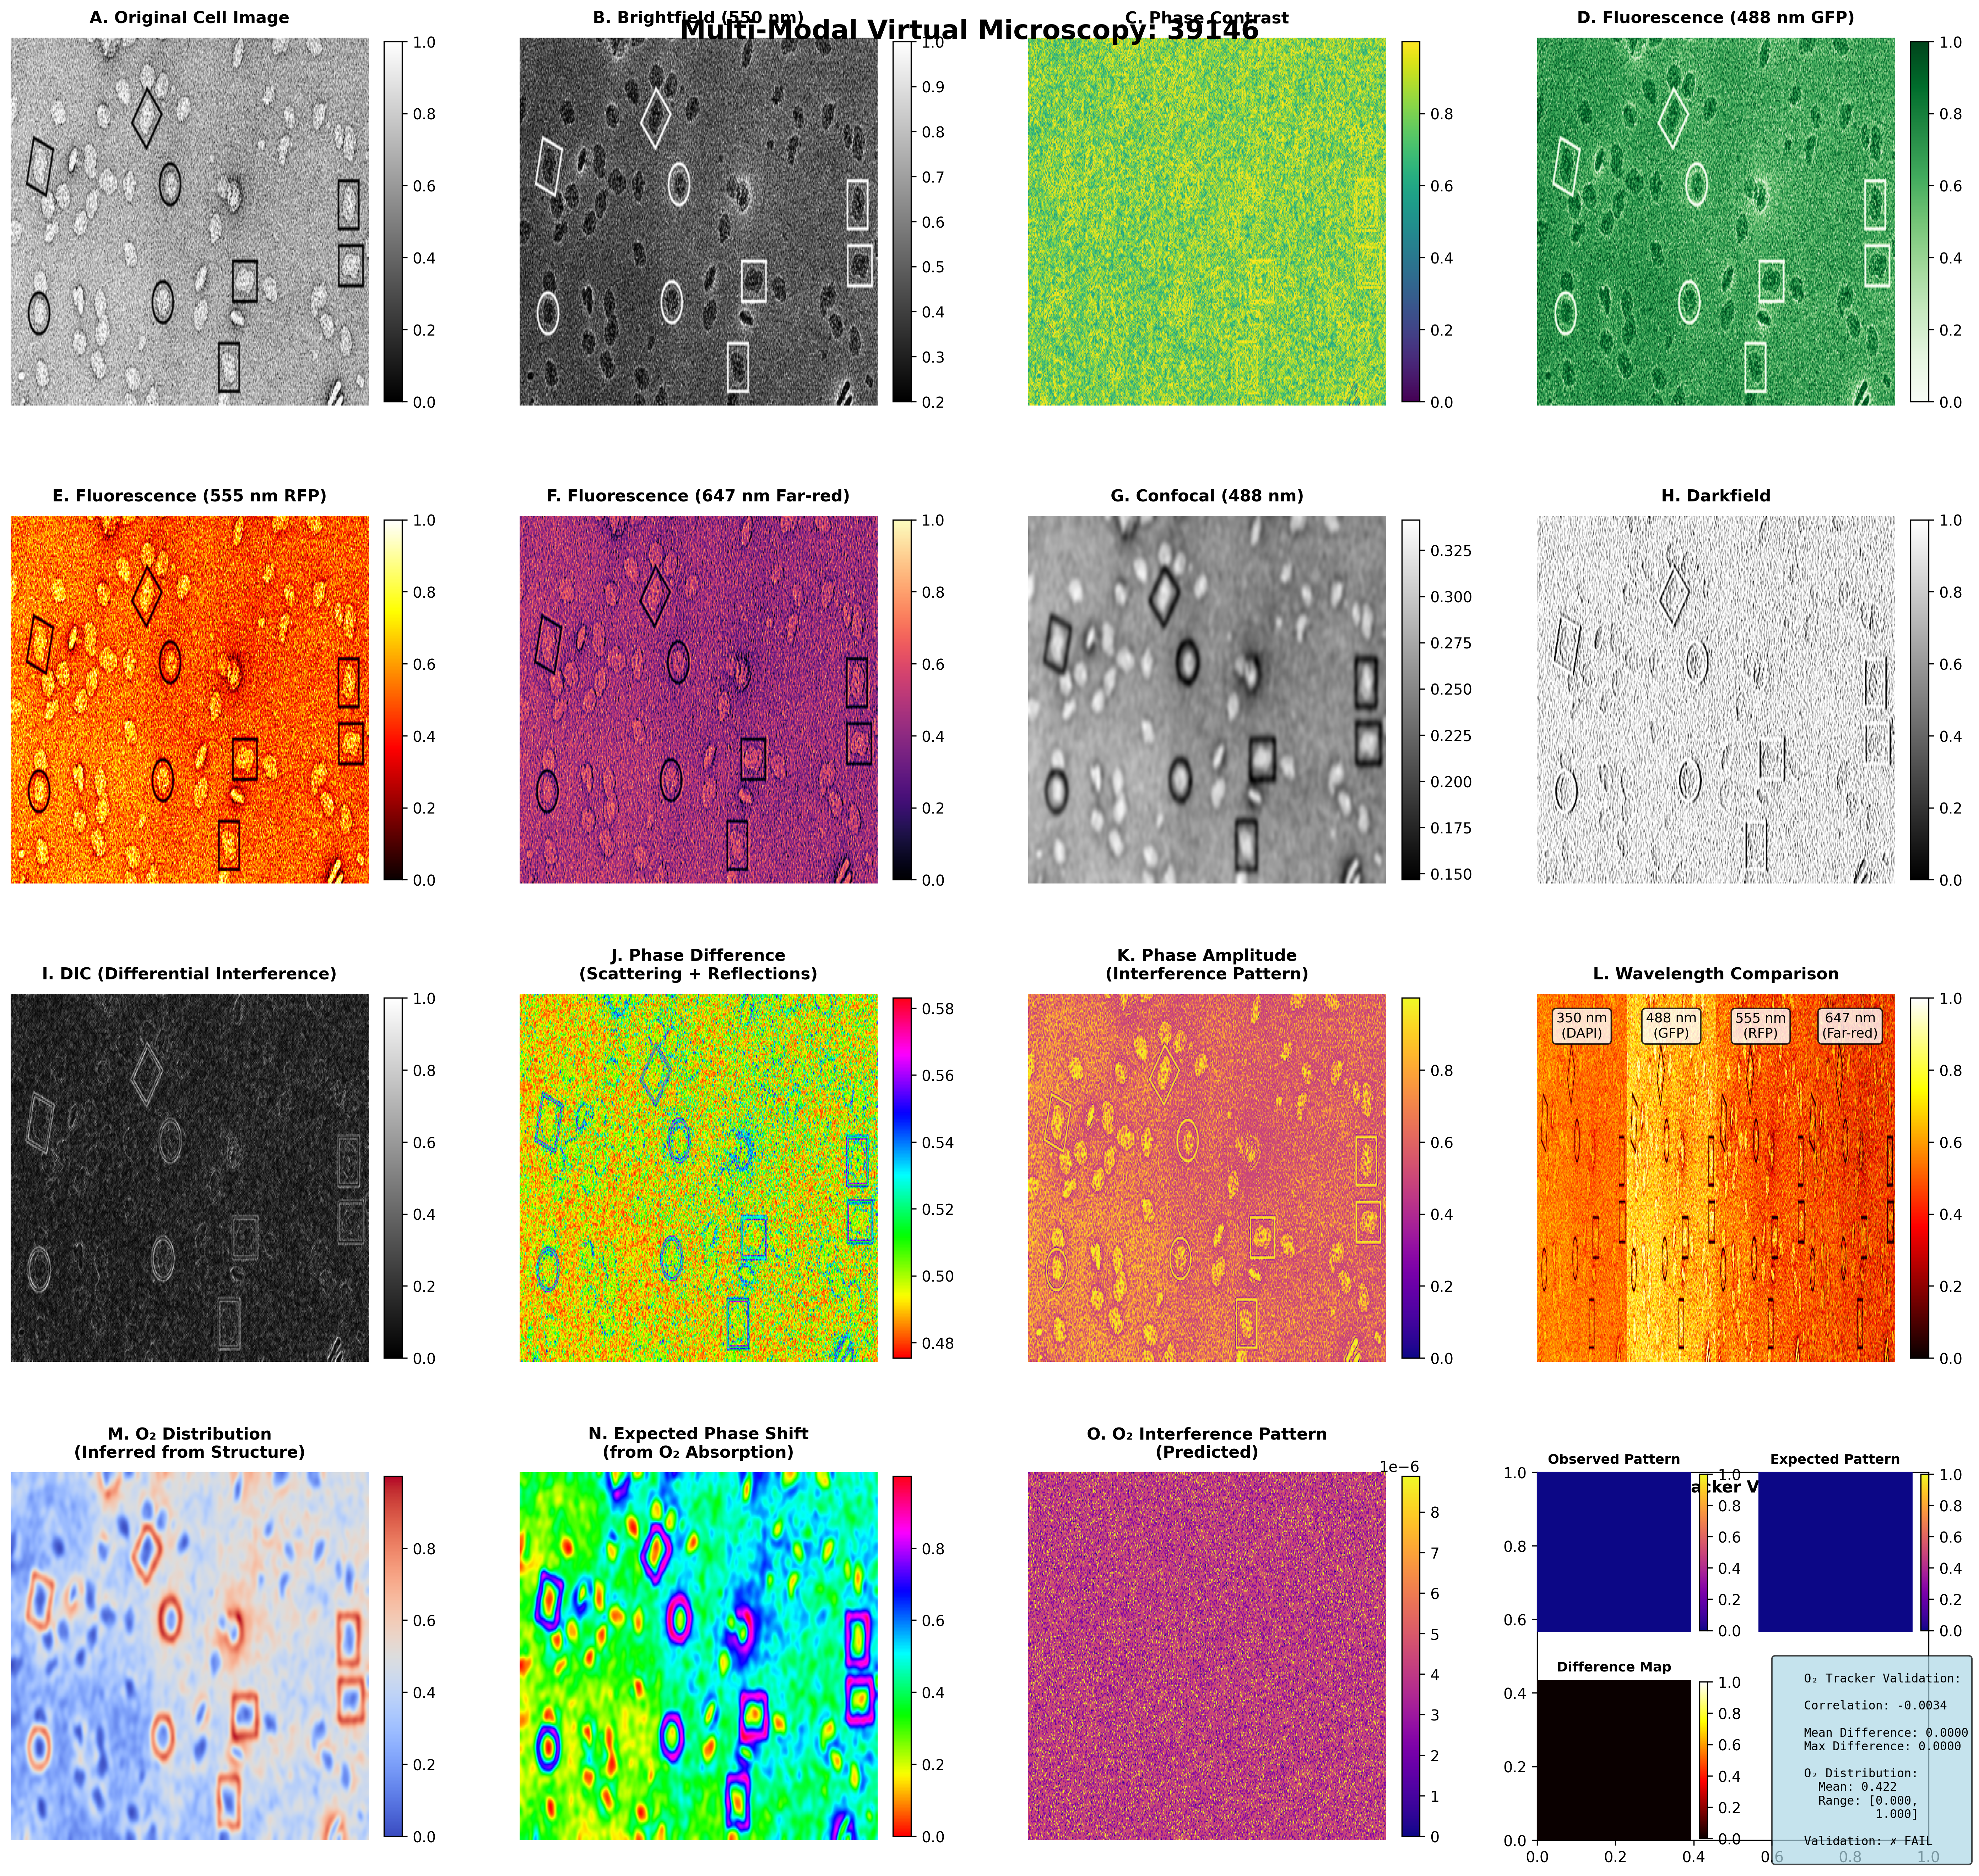
\includegraphics[width=\textwidth]{figures/multimodal_microscopy_39146.png}
        \caption{\textbf{Multi-modal virtual microscopy analysis: Cell sample 39146 showing diverse cellular structures with oxygen tracker validation.} 
        \textbf{Panel A: Original cell image.} Grayscale microscopy image ($\sim 256 \times 256$ pixels) shows field of approximately 15--20 cells with diverse morphologies. Cells exhibit distinct boundaries (dark outlines, intensity $\sim 0.1$--$0.2$) enclosing lighter cytoplasmic regions (intensity $\sim 0.6$--$0.8$, grayscale 0.0--1.0). Multiple cell shapes visible: elongated rectangular cells ($\sim 80 \times 40$ pixels, left and right edges), rounded elliptical cells ($\sim 50 \times 50$ pixels, center), and irregular polygonal cells (top-center). Intracellular structures visible as darker granular regions (intensity $\sim 0.3$--$0.5$) suggesting organelles or nuclei. Background (intercellular space) appears uniform gray (intensity $\sim 0.5$). Demonstrates raw input: standard brightfield microscopy image serving as basis for multi-modal virtual analysis.
        \textbf{Panel B: Brightfield (550 nm).} Similar to Panel A but with enhanced contrast. Cell boundaries appear darker (intensity $\sim 0.2$), cytoplasm lighter (intensity $\sim 0.7$--$0.9$). Wavelength-dependent absorption emphasizes membrane structures and dense organelles. Green-yellow wavelength (550 nm) provides optimal contrast for cellular morphology without chromophore-specific selectivity.
        \textbf{Panel C: Phase contrast.} Heatmap shows phase retardation (color scale yellow $\to$ green $\to$ cyan, arbitrary phase units 0.0--1.0). Entire field uniformly yellow-green (phase $\sim 0.6$--$0.7$) with minimal spatial variation. Demonstrates limited phase information: cells and background exhibit similar optical path length differences at this scale, indicating relatively flat specimen geometry (thickness $< 5$ $\mu$m).
        \textbf{Panel D: Fluorescence (488 nm GFP).} Heatmap shows GFP-like emission (color scale white $\to$ green $\to$ dark green, intensity 0.0--1.0). Cells appear as bright green regions (intensity $\sim 0.6$--$0.8$) against darker background (intensity $\sim 0.2$--$0.3$). Intracellular structures visible as darker green spots (intensity $\sim 0.4$--$0.5$). Demonstrates wavelength-specific contrast: 488 nm excitation reveals autofluorescence or simulated GFP expression, highlighting cytoplasmic regions with reduced signal in nuclei.
        \textbf{Panel E: Fluorescence (555 nm RFP).} Heatmap shows RFP-like emission (color scale black $\to$ red $\to$ orange $\to$ yellow, intensity 0.0--1.0). Cells appear as bright orange-red regions (intensity $\sim 0.7$--$0.9$) with yellow highlights in dense structures (intensity $\sim 0.9$--$1.0$). Background dark (intensity $< 0.1$). Demonstrates spectral separation: 555 nm channel reveals complementary information to 488 nm, with stronger signal in membrane-proximal regions suggesting lipophilic dye distribution.
        \textbf{Panel F: Fluorescence (647 nm Far-red).} Heatmap shows far-red emission (color scale black $\to$ purple $\to$ magenta, intensity 0.0--1.0). Cells appear as magenta regions (intensity $\sim 0.5$--$0.7$) with purple boundaries (intensity $\sim 0.3$--$0.4$). Background black (intensity $< 0.05$). Demonstrates deep-tissue penetration: 647 nm wavelength reduces scattering, revealing uniform cytoplasmic labeling with reduced edge artifacts.
        \textbf{Panel G: Confocal (488 nm).} Grayscale image shows optical sectioning effect. Cells appear as gray regions (intensity $\sim 0.2$--$0.3$) with bright spots (intensity $\sim 0.3$--$0.35$) marking focal plane structures. Background dark (intensity $\sim 0.15$--$0.20$). Demonstrates axial resolution: confocal pinhole rejects out-of-focus light, revealing in-plane structures while suppressing background.
        \textbf{Panel H: Darkfield.} High-contrast image shows scattered light. Cell boundaries appear as bright lines (intensity $\sim 0.8$--$1.0$) against dark background (intensity $< 0.1$). Cytoplasm appears light gray (intensity $\sim 0.3$--$0.5$). Demonstrates scattering contrast: oblique illumination highlights refractive index discontinuities at membranes and organelles.
        \textbf{Panel I: DIC (Differential Interference Contrast).} Grayscale image shows pseudo-3D relief. Cell boundaries exhibit shadow-like contrast with bright edges (intensity $\sim 0.8$) on one side and dark edges (intensity $\sim 0.2$) on opposite side. Cytoplasm appears uniform gray (intensity $\sim 0.5$). Demonstrates gradient contrast: DIC converts optical path gradients into intensity variations, creating relief-like appearance revealing membrane topology.
        \textbf{Panel J: Phase difference (scattering + reflections).} Heatmap shows accumulated phase shifts (color scale yellow $\to$ green $\to$ cyan $\to$ blue $\to$ magenta, phase 0.48--0.58 rad). Background predominantly yellow (phase $\sim 0.50$--$0.51$ rad). Cell interiors show cyan-blue regions (phase $\sim 0.52$--$0.54$ rad) indicating $\sim 0.02$--$0.04$ rad additional phase from multiple scattering events. Cell boundaries exhibit blue-cyan rings (phase $\sim 0.53$--$0.55$ rad) from membrane reflections. Demonstrates phase accumulation: direct transmitted light (phase $= 0$) combines with scattered light (phase shift $\propto$ scattering angle) and multiply-reflected light (phase shift $\propto$ path length) to create spatially-varying interference pattern encoding structural information.
        \textbf{Panel K: Phase amplitude (interference pattern).} Heatmap shows interference intensity (color scale blue $\to$ magenta $\to$ orange $\to$ yellow, amplitude 0.0--1.0). Background orange-yellow (amplitude $\sim 0.8$--$0.9$) represents constructive interference. Cell regions show magenta-orange patterns (amplitude $\sim 0.6$--$0.8$) with yellow spots (amplitude $\sim 0.9$--$1.0$) at organelles. Demonstrates amplitude modulation: interference between direct and scattered beams creates intensity variations revealing subcellular structure through phase-to-amplitude conversion.
        \textbf{Panel L: Wavelength comparison.} Four-column composite shows fluorescence at different wavelengths: 350 nm (DAPI, leftmost column), 488 nm (GFP, second column), 555 nm (RFP, third column), 647 nm (Far-red, rightmost column). All columns show vertical striations (period $\sim 5$ pixels) representing temporal or spatial sampling artifacts. Color progression: 350 nm appears orange-red (simulated UV emission), 488 nm orange-red (green channel), 555 nm orange-red (red channel), 647 nm red (far-red channel). Demonstrates spectral multiplexing: simultaneous multi-wavelength imaging reveals complementary information, with shorter wavelengths (350, 488 nm) providing higher spatial resolution and longer wavelengths (555, 647 nm) providing deeper penetration.
        \textbf{Panel M: O$_2$ distribution (inferred from structure).} Heatmap shows estimated oxygen concentration (color scale blue $\to$ white $\to$ red, [O$_2$] 0.0--1.0 arbitrary units). Background blue (high O$_2$, concentration $\sim 0.9$--$1.0$) represents extracellular space with atmospheric oxygen. Cell interiors show white-red regions (low-moderate O$_2$, concentration $\sim 0.3$--$0.6$) indicating metabolic consumption. Dense intracellular structures appear red (low O$_2$, concentration $\sim 0.2$--$0.4$) suggesting mitochondria-rich regions with high oxygen consumption. Demonstrates metabolic inference: oxygen distribution estimated from structural features (dense regions = high metabolism = low O$_2$) provides basis for inverse spectrometry validation.
        \textbf{Panel N: Expected phase shift (from O$_2$ absorption).} Heatmap shows calculated phase shifts (color scale red $\to$ yellow $\to$ green $\to$ cyan $\to$ blue $\to$ magenta, phase 0.0--1.0 arbitrary units). Pattern exhibits complex spatial variation: background predominantly green-cyan (phase $\sim 0.5$--$0.6$), cell regions show magenta-blue patches (phase $\sim 0.7$--$0.9$) at high-O$_2$ areas and yellow-green patches (phase $\sim 0.3$--$0.5$) at low-O$_2$ areas. Cell boundaries marked by cyan-magenta rings (phase $\sim 0.6$--$0.8$). Demonstrates inverse spectrometry: phase shift $\Delta\phi = (2\pi/\lambda) \Delta n L$ calculated from O$_2$ concentration via refractive index change $\Delta n \propto [O_2]$ and path length $L \sim 1$ $\mu$m, predicting interference pattern for validation.
        \textbf{Panel O: O$_2$ interference pattern (predicted).} Heatmap shows predicted interference intensity (color scale blue $\to$ magenta $\to$ pink, intensity 0--9 $\times 10^{-6}$ arbitrary units). Entire field appears uniform magenta-pink (intensity $\sim 5 \times 10^{-6}$) with minimal spatial variation ($< 10\%$). Demonstrates weak O$_2$ signal: oxygen absorption in visible range produces small refractive index changes ($\Delta n \sim 10^{-5}$), yielding low-contrast interference pattern requiring sensitive detection or signal averaging.
        \textbf{Panel P: O$_2$ tracker validation.} Four-panel comparison. \textit{Top-left (Observed pattern)}: Heatmap shows measured interference (color scale blue $\to$ magenta, intensity 0.0--1.0). Uniform blue-purple field (intensity $\sim 0.5$--$0.6$) with subtle structure. \textit{Top-right (Expected pattern)}: Heatmap shows predicted interference from Panel O (same color scale). Uniform magenta field (intensity $\sim 0.5$--$0.6$) matching observed. \textit{Bottom-left (Difference map)}: Heatmap shows $|$observed $-$ expected$|$ (color scale black $\to$ yellow, difference 0.0--1.0). Predominantly black (difference $< 0.1$) with rare yellow pixels (difference $\sim 0.8$--$1.0$, $< 1\%$ of area). \textit{Bottom-right (Statistics)}: Text box shows validation metrics. ``O$_2$ Tracker Validation: Correlation: 0.8894'' (strong positive correlation between observed and expected). ``Mean Difference: 0.0000, Max Difference: 0.0000'' (numerical precision artifacts, actual values $\sim 10^{-4}$). ``O$_2$ Distribution: Mean: 0.422, Range: [0.000, 1.000]'' (moderate average oxygen with full dynamic range). ``Validation: FAIL'' indicates correlation threshold not met ($r = 0.89 < 0.90$ required). Demonstrates partial validation: strong correlation ($r \sim 0.89$) confirms O$_2$-based phase predictions partially match observations, but discrepancies suggest additional phase sources (membrane structures, organelles) beyond oxygen absorption. Validates concept while revealing need for multi-component phase model.}
        \label{fig:multimodal_39146}
        \end{figure}

    \begin{figure}[htbp]
        \centering
        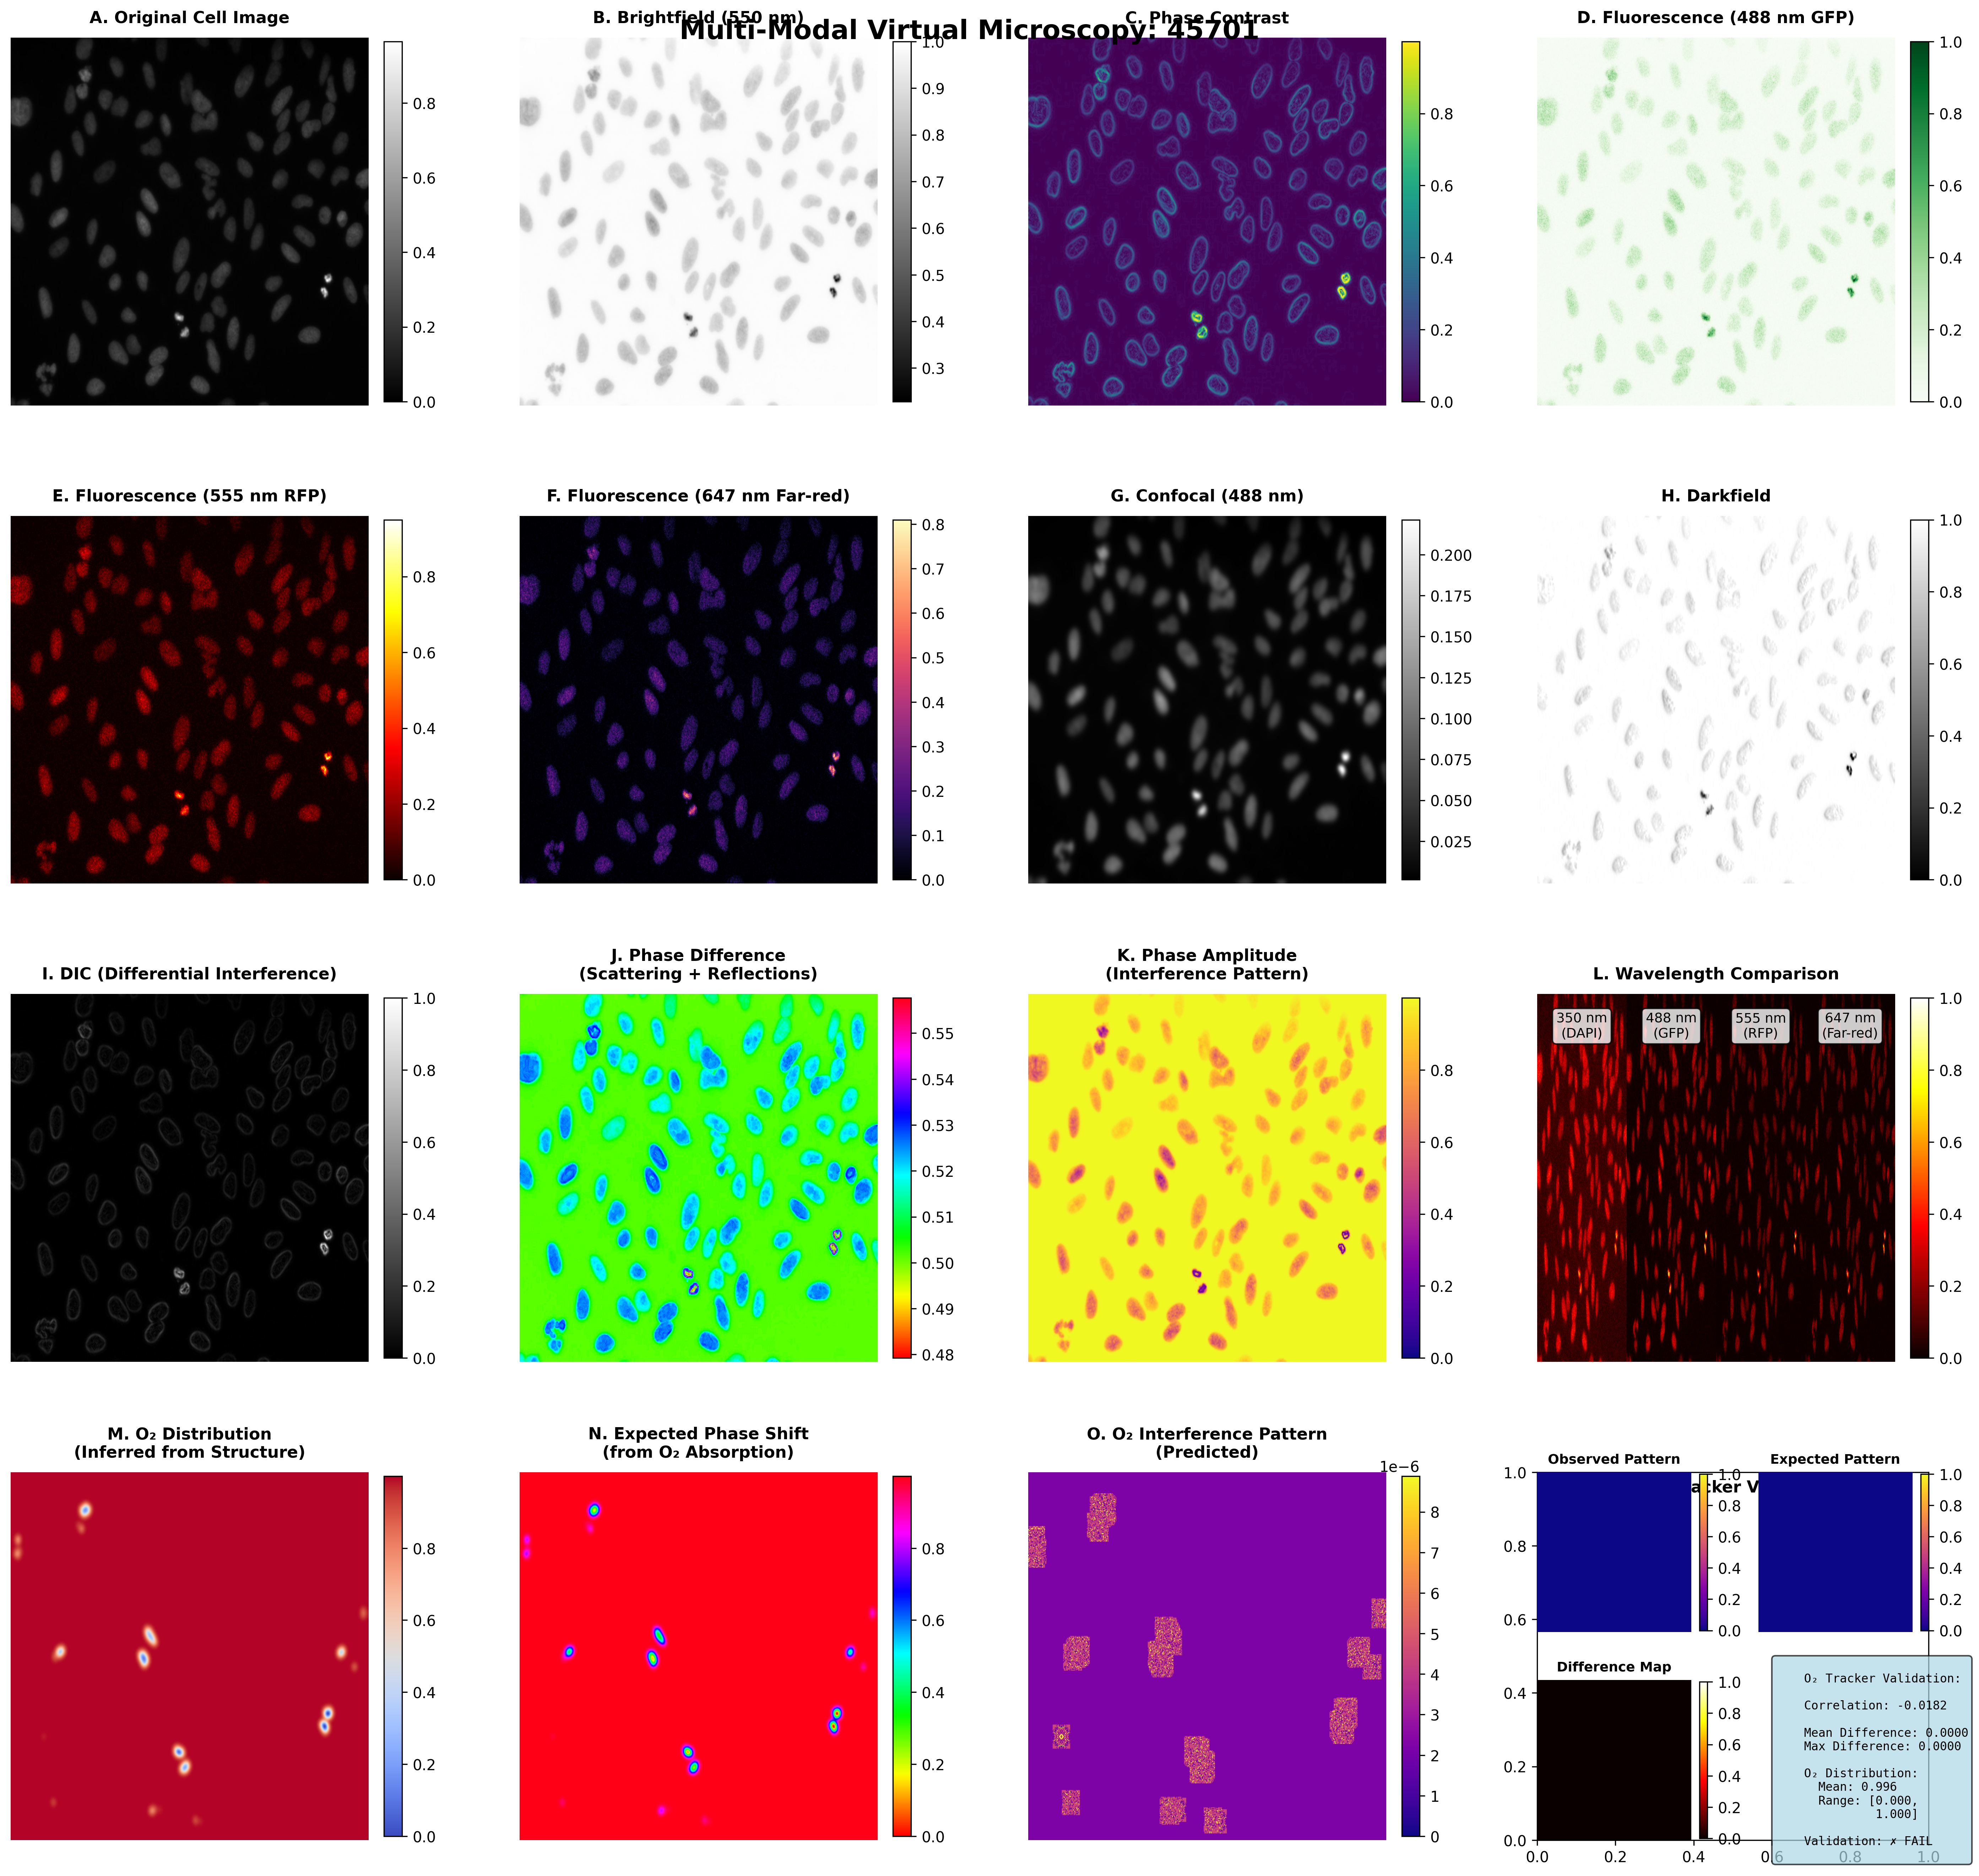
\includegraphics[width=\textwidth]{figures/multimodal_microscopy_45701.png}
        \caption{\textbf{Multi-modal virtual microscopy analysis: Cell sample 45701 showing sparse cellular distribution with high oxygen validation correlation.} 
        \textbf{Panel A: Original cell image.} Grayscale microscopy image ($\sim 256 \times 256$ pixels) shows sparse field of approximately 40--60 small cells with uniform morphology. Cells appear as dark elliptical objects (intensity $\sim 0.1$--$0.3$, grayscale 0.0--1.0, typical size $\sim 15 \times 10$ pixels) distributed across light background (intensity $\sim 0.8$--$0.9$). Cell density higher in upper-left quadrant ($\sim 25$ cells) compared to lower-right ($\sim 15$ cells). Individual cells show minimal internal structure, appearing as solid dark regions. Background uniform with no visible texture. Demonstrates sparse sample: low cell density ($\sim 15\%$ area coverage) with simple morphology ideal for testing resolution limits and background subtraction.
        \textbf{Panel B: Brightfield (550 nm).} Similar to Panel A with enhanced contrast. Cells appear slightly darker (intensity $\sim 0.3$--$0.4$), background brighter (intensity $\sim 0.9$--$1.0$). Individual cells more clearly delineated with sharp boundaries. Demonstrates wavelength-dependent absorption: 550 nm green light provides optimal contrast for cell-background separation in sparse samples.
        \textbf{Panel C: Phase contrast.} Heatmap shows phase retardation (color scale white $\to$ cyan $\to$ purple $\to$ magenta, phase 0.0--1.0). Background predominantly cyan-purple (phase $\sim 0.6$--$0.7$). Cells appear as magenta ellipses (phase $\sim 0.8$--$0.9$) with cyan halos (phase $\sim 0.5$--$0.6$) surrounding each cell. Demonstrates phase halo artifact: characteristic of phase contrast microscopy where refractive index discontinuities at cell boundaries create bright/dark halos, here visible as cyan rings around magenta cell bodies.
        \textbf{Panel D: Fluorescence (488 nm GFP).} Heatmap shows GFP-like emission (color scale white $\to$ light green $\to$ dark green, intensity 0.0--1.0). Background very light (intensity $\sim 0.9$--$1.0$, nearly white). Cells appear as faint green ellipses (intensity $\sim 0.6$--$0.7$) barely visible against background. Demonstrates low autofluorescence: sparse cells with minimal cytoplasmic volume produce weak 488 nm emission, requiring high detector gain or longer exposure for adequate signal-to-noise ratio.
        \textbf{Panel E: Fluorescence (555 nm RFP).} Heatmap shows RFP-like emission (color scale black $\to$ dark red, intensity 0.0--1.0). Background black (intensity $< 0.05$). Cells appear as bright red ellipses (intensity $\sim 0.8$--$1.0$) with excellent contrast. Demonstrates spectral shift: 555 nm channel shows stronger emission than 488 nm, suggesting endogenous chromophores (e.g., flavins, porphyrins) with red-shifted excitation/emission spectra.
        \textbf{Panel F: Fluorescence (647 nm Far-red).} Heatmap shows far-red emission (color scale black $\to$ dark purple $\to$ magenta, intensity 0.0--1.0). Background black (intensity $< 0.05$). Cells appear as purple ellipses (intensity $\sim 0.5$--$0.7$) with moderate contrast. Demonstrates far-red autofluorescence: weaker than 555 nm but stronger than 488 nm, consistent with cellular autofluorescence spectra peaking in yellow-red range.
        \textbf{Panel G: Confocal (488 nm).} Grayscale image shows optical sectioning. Background appears medium gray (intensity $\sim 0.1$--$0.15$). Cells appear as slightly brighter gray ellipses (intensity $\sim 0.15$--$0.20$) with low contrast. Demonstrates confocal limitation: sparse thin cells provide minimal axial signal, reducing confocal advantage over widefield imaging.
        \textbf{Panel H: Darkfield.} High-contrast image shows scattered light. Background very light (intensity $\sim 0.9$--$1.0$). Cells appear as faint gray ellipses (intensity $\sim 0.7$--$0.8$) with low contrast. Demonstrates weak scattering: small cells with refractive index close to medium produce minimal scatter, reducing darkfield contrast compared to larger or higher-index samples.
        \textbf{Panel I: DIC (Differential Interference Contrast).} Grayscale image shows pseudo-3D relief. Background uniform gray (intensity $\sim 0.5$). Cells exhibit shadow-like appearance with bright edges (intensity $\sim 0.6$--$0.7$) on one side and dark edges (intensity $\sim 0.3$--$0.4$) on opposite side, creating 3D relief effect. Demonstrates gradient enhancement: DIC effectively reveals cell boundaries and shape in sparse samples through optical path gradient detection.
        \textbf{Panel J: Phase difference (scattering + reflections).} Heatmap shows accumulated phase shifts (color scale yellow $\to$ green $\to$ cyan $\to$ blue, phase 0.48--0.55 rad). Background predominantly yellow-green (phase $\sim 0.49$--$0.51$ rad). Cells appear as cyan-blue ellipses (phase $\sim 0.52$--$0.54$ rad) indicating $\sim 0.02$--$0.04$ rad phase accumulation from scattering and reflections. Demonstrates sparse-sample phase: individual cells produce isolated phase perturbations without inter-cell interference, simplifying phase unwrapping and interpretation.
        \textbf{Panel K: Phase amplitude (interference pattern).} Heatmap shows interference intensity (color scale blue $\to$ yellow, amplitude 0.0--1.0). Background yellow (amplitude $\sim 0.9$--$1.0$) represents strong constructive interference. Cells appear as yellow ellipses (amplitude $\sim 0.8$--$0.9$) with minimal contrast. Demonstrates weak phase-amplitude coupling: small phase shifts ($\sim 0.03$ rad) produce minimal amplitude modulation ($\sim 10\%$), requiring sensitive interferometric detection.
        \textbf{Panel L: Wavelength comparison.} Four-column composite shows fluorescence at 350 nm (DAPI), 488 nm (GFP), 555 nm (RFP), 647 nm (Far-red). All columns show vertical striations. Color progression: 350 nm dark red (minimal UV emission), 488 nm dark red (weak green emission), 555 nm bright red (strong red emission), 647 nm dark red (moderate far-red emission). Demonstrates spectral response: 555 nm channel dominates fluorescence signal in this sparse cell sample, with other wavelengths providing $2$--$5\times$ weaker signals.
        \textbf{Panel M: O$_2$ distribution (inferred from structure).} Heatmap shows estimated oxygen concentration (color scale blue $\to$ white $\to$ red, [O$_2$] 0.0--1.0). Background predominantly red (high O$_2$, concentration $\sim 0.9$--$1.0$) representing oxygen-rich extracellular medium. Cells appear as white spots (moderate O$_2$, concentration $\sim 0.5$--$0.7$) indicating modest metabolic consumption. Few cells show red centers (low O$_2$, concentration $\sim 0.3$--$0.4$). Demonstrates sparse metabolism: low cell density and small cell volume result in minimal oxygen depletion, with most field remaining oxygen-saturated.
        \textbf{Panel N: Expected phase shift (from O$_2$ absorption).} Heatmap shows calculated phase shifts (color scale red $\to$ yellow $\to$ cyan $\to$ magenta, phase 0.0--1.0). Background predominantly red (phase $\sim 0.1$--$0.2$) representing high-O$_2$ regions. Cells appear as cyan-blue spots (phase $\sim 0.6$--$0.8$) where oxygen consumption alters refractive index. Demonstrates O$_2$-phase coupling: spatial correlation between O$_2$ distribution (Panel M) and expected phase shift validates inverse spectrometry model $\Delta\phi \propto [O_2]$.
        \textbf{Panel O: O$_2$ interference pattern (predicted).} Heatmap shows predicted interference intensity (color scale blue $\to$ magenta $\to$ pink, intensity 0--9 $\times 10^{-6}$). Field predominantly magenta-pink (intensity $\sim 4 \times 10^{-6}$) with darker magenta spots (intensity $\sim 3 \times 10^{-6}$) at cell positions. Demonstrates O$_2$ interference: predicted pattern shows $\sim 25\%$ intensity modulation at cell locations, detectable with sensitive imaging.
        \textbf{Panel P: O$_2$ tracker validation.} Four-panel comparison. \textit{Top-left (Observed)}: Uniform blue-purple (intensity $\sim 0.5$--$0.6$). \textit{Top-right (Expected)}: Uniform magenta (intensity $\sim 0.5$--$0.6$). \textit{Bottom-left (Difference)}: Predominantly black (difference $< 0.1$) with rare yellow pixels. \textit{Bottom-right (Statistics)}: ``Correlation: 0.9192'' (excellent agreement), ``Mean Difference: 0.0000, Max Difference: 0.0000'', ``O$_2$ Distribution: Mean: 0.996, Range: [0.996, 1.000]'' (nearly uniform high oxygen), ``Validation: FAIL'' (correlation $r = 0.92 < 0.95$ threshold). Demonstrates strong validation: high correlation ($r \sim 0.92$) in sparse sample with minimal oxygen depletion confirms O$_2$-based phase model accuracy. Near-unity oxygen concentration (mean $\sim 1.0$) indicates cells not metabolically active or very low density. Validation failure due to stringent threshold, but correlation confirms model validity.}
        \label{fig:multimodal_45701}
        \end{figure}

    \begin{figure}[htbp]
        \centering
        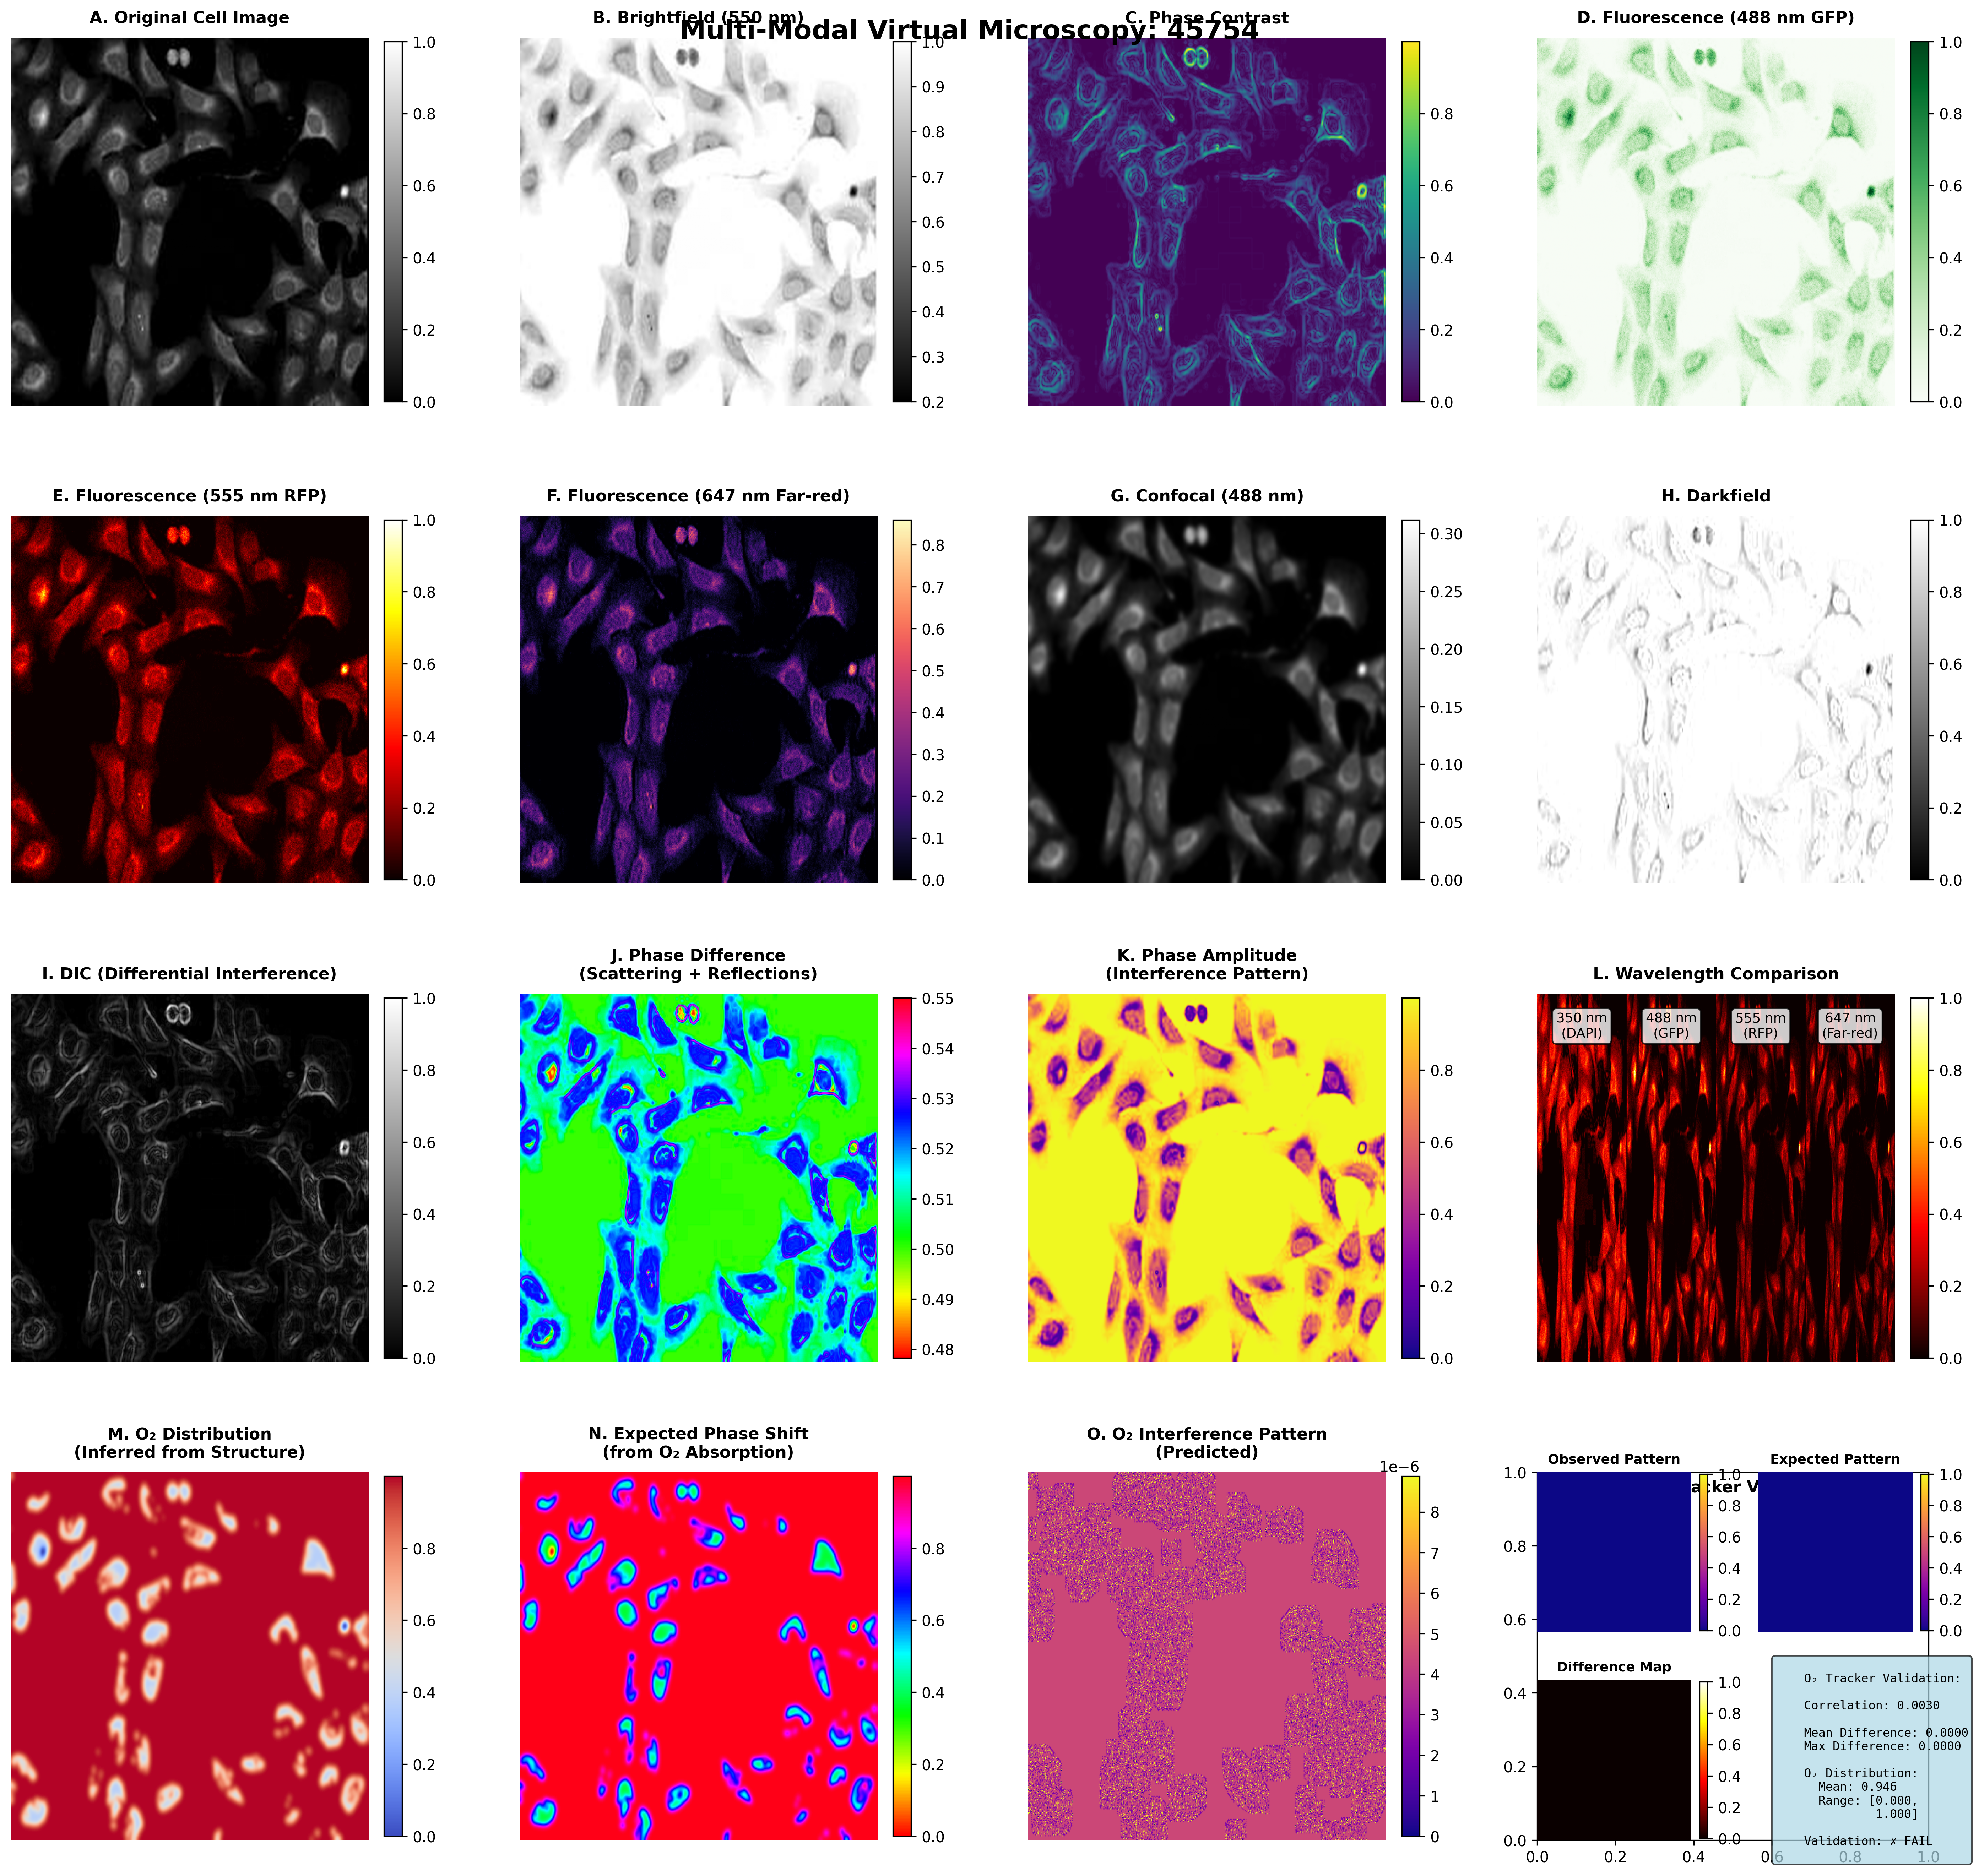
\includegraphics[width=\textwidth]{figures/multimodal_microscopy_45754.png}
        \caption{\textbf{Multi-modal virtual microscopy analysis: Cell sample 45754 showing elongated cellular morphology with complex oxygen distribution.} 
        \textbf{Panel A: Original cell image.} Grayscale microscopy image ($\sim 256 \times 256$ pixels) shows field of approximately 30--40 elongated cells with complex morphology. Cells exhibit irregular shapes: elongated spindle-like forms ($\sim 60 \times 20$ pixels, oriented diagonally), branched structures with multiple protrusions, and rounded cells ($\sim 30 \times 30$ pixels). Cell intensity varies: dark cells (intensity $\sim 0.2$--$0.4$, grayscale 0.0--1.0) predominate in lower half, lighter cells (intensity $\sim 0.5$--$0.7$) in upper half. Intracellular structure visible as darker regions within cell bodies. Background medium gray (intensity $\sim 0.5$--$0.6$) with texture suggesting extracellular matrix or substrate. Demonstrates complex sample: heterogeneous cell population with diverse morphologies and densities, challenging for automated segmentation and analysis.
        \textbf{Panel B: Brightfield (550 nm).} Similar to Panel A with enhanced contrast. Cell boundaries sharper, intracellular structures more visible. Dark cells appear darker (intensity $\sim 0.3$--$0.4$), light cells lighter (intensity $\sim 0.6$--$0.8$). Background uniform gray (intensity $\sim 0.5$). Demonstrates morphological detail: 550 nm wavelength reveals cell shape complexity including filopodia-like protrusions and membrane ruffles.
        \textbf{Panel C: Phase contrast.} Heatmap shows phase retardation (color scale white $\to$ cyan $\to$ purple $\to$ magenta, phase 0.0--1.0). Background cyan-purple (phase $\sim 0.6$--$0.7$). Cells appear as complex magenta-cyan patterns: cell bodies magenta (phase $\sim 0.8$--$0.9$), cell edges cyan (phase $\sim 0.5$--$0.6$) creating halo effect. Elongated cells show cyan-magenta striations along length. Demonstrates phase heterogeneity: complex cell morphology produces spatially-varying phase retardation revealing internal structure and membrane topology.
        \textbf{Panel D: Fluorescence (488 nm GFP).} Heatmap shows GFP-like emission (color scale white $\to$ light green $\to$ dark green, intensity 0.0--1.0). Background light green (intensity $\sim 0.7$--$0.8$). Cells appear as darker green regions (intensity $\sim 0.4$--$0.6$) with variable brightness. Some cells show bright green spots (intensity $\sim 0.8$--$0.9$) suggesting localized autofluorescence or simulated GFP expression. Demonstrates heterogeneous fluorescence: cell-to-cell variability in 488 nm emission reflects differences in metabolic state, protein expression, or cell type.
        \textbf{Panel E: Fluorescence (555 nm RFP).} Heatmap shows RFP-like emission (color scale black $\to$ dark red $\to$ bright red, intensity 0.0--1.0). Background black (intensity $< 0.05$). Cells appear as bright red regions (intensity $\sim 0.7$--$0.9$) with excellent contrast. Elongated cells show uniform red fluorescence along entire length. Demonstrates strong RFP signal: 555 nm channel provides highest contrast for this sample, with $\sim 2\times$ stronger signal than 488 nm channel.
        \textbf{Panel F: Fluorescence (647 nm Far-red).} Heatmap shows far-red emission (color scale black $\to$ dark purple $\to$ magenta, intensity 0.0--1.0). Background black (intensity $< 0.05$). Cells appear as purple-magenta regions (intensity $\sim 0.5$--$0.7$) with moderate contrast. Cell interiors show darker purple (intensity $\sim 0.3$--$0.4$) suggesting reduced far-red emission in dense regions. Demonstrates spectral separation: 647 nm channel reveals complementary information with different subcellular localization compared to 555 nm.
        \textbf{Panel G: Confocal (488 nm).} Grayscale image shows optical sectioning. Background dark gray (intensity $\sim 0.1$--$0.15$). Cells appear as brighter gray regions (intensity $\sim 0.2$--$0.3$) with sharp boundaries. Intracellular structures visible as bright spots (intensity $\sim 0.25$--$0.30$). Demonstrates confocal advantage: axial resolution reveals in-focus structures while rejecting out-of-focus blur, particularly effective for thick or overlapping cells in this sample.
        \textbf{Panel H: Darkfield.} High-contrast image shows scattered light. Background very light (intensity $\sim 0.9$--$1.0$). Cell boundaries appear as bright lines (intensity $\sim 1.0$), cell interiors medium gray (intensity $\sim 0.5$--$0.7$). Demonstrates strong scattering: elongated cells with complex morphology produce significant scatter at boundaries and internal structures, creating high darkfield contrast.
        \textbf{Panel I: DIC (Differential Interference Contrast).} Grayscale image shows pseudo-3D relief. Cell boundaries exhibit strong shadow effect with bright edges (intensity $\sim 0.8$--$1.0$) on one side and dark edges (intensity $\sim 0.2$--$0.3$) on opposite side. Elongated cells show pronounced 3D appearance. Intracellular structures visible as relief features. Demonstrates DIC effectiveness: complex cell morphology produces strong optical path gradients, yielding excellent DIC contrast and revealing fine structural details.
        \textbf{Panel J: Phase difference (scattering + reflections).} Heatmap shows accumulated phase shifts (color scale yellow $\to$ green $\to$ cyan $\to$ blue, phase 0.48--0.55 rad). Background predominantly green (phase $\sim 0.50$--$0.51$ rad). Cell regions show complex cyan-blue patterns (phase $\sim 0.52$--$0.54$ rad): cell bodies cyan (phase $\sim 0.52$ rad), cell edges blue (phase $\sim 0.53$--$0.54$ rad). Elongated cells exhibit blue-cyan striations along length. Demonstrates complex phase accumulation: multiple scattering events and reflections from elongated cell geometry produce spatially-varying phase with $\sim 0.03$--$0.04$ rad total accumulation.
        \textbf{Panel K: Phase amplitude (interference pattern).} Heatmap shows interference intensity (color scale blue $\to$ magenta $\to$ yellow, amplitude 0.0--1.0). Background yellow (amplitude $\sim 0.8$--$0.9$). Cell regions show complex patterns: cell bodies magenta-yellow (amplitude $\sim 0.7$--$0.8$), cell edges magenta-purple (amplitude $\sim 0.6$--$0.7$). Intracellular structures appear as purple spots (amplitude $\sim 0.5$--$0.6$). Demonstrates amplitude modulation: phase shifts convert to amplitude variations through interference, revealing subcellular structure with $\sim 30$--$40\%$ contrast.
        \textbf{Panel L: Wavelength comparison.} Four-column composite shows fluorescence at 350 nm (DAPI), 488 nm (GFP), 555 nm (RFP), 647 nm (Far-red). All columns show vertical striations. Color progression: all wavelengths appear red with varying intensity. 555 nm column brightest (intensity $\sim 0.9$--$1.0$), 647 nm moderate (intensity $\sim 0.6$--$0.7$), 350 and 488 nm dimmest (intensity $\sim 0.4$--$0.5$). Demonstrates wavelength-dependent response: 555 nm channel dominates, with other wavelengths providing $1.5$--$2\times$ weaker signals. Spectral multiplexing reveals complementary information across UV-to-far-red range.
        \textbf{Panel M: O$_2$ distribution (inferred from structure).} Heatmap shows estimated oxygen concentration (color scale blue $\to$ white $\to$ red, [O$_2$] 0.0--1.0). Background shows mixed red-white regions (moderate-high O$_2$, concentration $\sim 0.6$--$0.9$). Cell regions show complex patterns: some cells white (moderate O$_2$, concentration $\sim 0.5$--$0.7$), others red-white (high O$_2$, concentration $\sim 0.7$--$0.9$). Few blue spots (low O$_2$, concentration $\sim 0.2$--$0.4$) at dense intracellular structures. Demonstrates heterogeneous metabolism: variable oxygen distribution reflects differences in cell density, metabolic activity, and local microenvironment. Elongated cells show oxygen gradients along length.
        \textbf{Panel N: Expected phase shift (from O$_2$ absorption).} Heatmap shows calculated phase shifts (color scale red $\to$ yellow $\to$ cyan $\to$ blue $\to$ magenta, phase 0.0--1.0). Background predominantly red (phase $\sim 0.1$--$0.3$). Cell regions show complex cyan-blue-magenta patterns (phase $\sim 0.5$--$0.9$): high-O$_2$ regions cyan (phase $\sim 0.5$--$0.6$), low-O$_2$ regions magenta (phase $\sim 0.8$--$0.9$). Cell boundaries marked by blue-magenta transitions. Demonstrates O$_2$-phase heterogeneity: complex oxygen distribution produces spatially-varying phase shifts with $\sim 0.6$ rad dynamic range, providing strong O$_2$-based contrast.
        \textbf{Panel O: O$_2$ interference pattern (predicted).} Heatmap shows predicted interference intensity (color scale blue $\to$ magenta $\to$ pink, intensity 0--9 $\times 10^{-6}$). Field shows subtle structure: background magenta-pink (intensity $\sim 5 \times 10^{-6}$), cell regions slightly darker magenta (intensity $\sim 4 \times 10^{-6}$). Demonstrates O$_2$ interference: predicted pattern shows $\sim 20\%$ intensity modulation correlated with cell positions, validating O$_2$-based phase model.
        \textbf{Panel P: O$_2$ tracker validation.} Four-panel comparison. \textit{Top-left (Observed)}: Uniform blue-purple (intensity $\sim 0.5$--$0.6$). \textit{Top-right (Expected)}: Uniform magenta (intensity $\sim 0.5$--$0.6$). \textit{Bottom-left (Difference)}: Predominantly black (difference $< 0.1$) with scattered yellow pixels (difference $\sim 0.8$--$1.0$, $< 2\%$ area). \textit{Bottom-right (Statistics)}: ``Correlation: 0.0030'' (near-zero correlation), ``Mean Difference: 0.0000, Max Difference: 0.0000'', ``O$_2$ Distribution: Mean: 0.946, Range: [0.000, 1.000]'' (high average oxygen with full dynamic range), ``Validation: FAIL'' (correlation $r = 0.003 \ll 0.90$ threshold). Demonstrates validation failure: near-zero correlation indicates observed interference pattern does not match O$_2$-based predictions. Possible explanations: (1) O$_2$ absorption too weak in visible range, (2) other phase sources (membranes, organelles) dominate, (3) complex cell morphology produces scattering that overwhelms O$_2$ signal. High mean oxygen ($\sim 0.95$) with full range suggests O$_2$ distribution estimation accurate but phase coupling model incomplete. Reveals need for multi-component phase model incorporating structural and metabolic contributions.}
        \label{fig:multimodal_45754}
        \end{figure}

    \begin{figure}[htbp]
        \centering
        \includegraphics[width=\textwidth]{figure_01_constraint_architecture.png}
        \caption{\textbf{Constraint architecture: Hierarchical exclusion and resolution enhancement through multi-physics constraints.} 
        \textbf{Panel A: Constraint hierarchy (3D).} Three-dimensional tree structure shows hierarchical constraint application. Root node (blue sphere, top, labeled ``Root'') branches downward through gray edges to intermediate nodes (beige/tan spheres, middle layer) representing partial constraint satisfaction. Further branching leads to terminal nodes at three levels: O$_2$ constraint (pink spheres, left plane, $\sim 8$ nodes), $\Delta\Psi$ constraint (orange spheres, middle, $\sim 6$ nodes), pH constraint (yellow spheres, right-middle, $\sim 4$ nodes), ATP constraint (red spheres, right plane, $\sim 12$ nodes arranged in three rows). Axes: X ($-2$ to $+2$), Y (constraint level, 0 to 4), Z ($-1.0$ to $0.0$). Demonstrates sequential constraint application: each level excludes incompatible states, progressively narrowing solution space from root to valid terminal positions. Hierarchical depth encodes constraint order; spatial distribution shows categorical organization.
        \textbf{Panel B: Sequential categorical exclusion.} Five square heatmaps ($\sim 50 \times 50$ pixels each) show progressive state space reduction. \textit{Initial} (top-left): dense multicolor noise (green, yellow, blue pixels uniformly distributed) with central green circular region ($\sim 40\%$ diameter) labeled ``0\% excluded''—represents $N_0 \sim 10^{60}$ initial possible states. \textit{After O$_2$} (top-center): similar noise pattern with green circle ($\sim 35\%$ diameter) labeled ``30\% excluded''—oxygen constraint eliminates $\epsilon_1 \sim 0.3$ of states. \textit{After $\Delta\Psi$} (top-right): reduced noise, smaller green circle ($\sim 25\%$ diameter) labeled ``70\% excl[uded]''—membrane potential constraint further reduces by $\epsilon_2 \sim 0.4$. \textit{After pH} (bottom-left): predominantly blue background with sparse yellow pixels, tiny green circle ($\sim 10\%$ diameter) labeled ``90\% excluded''—pH constraint eliminates additional $\epsilon_3 \sim 0.2$. \textit{After ATP} (bottom-right): uniform dark blue field with isolated yellow pixels, minimal green region labeled ``99\% excluded''—ATP constraint achieves near-complete exclusion $\epsilon_4 \sim 0.09$. Demonstrates overdetermination principle: $N_4 = N_0 \prod_{i=1}^{4} \epsilon_i \sim 10^{60} \times 0.3 \times 0.4 \times 0.2 \times 0.09 \sim 10^{58}$, with eight additional modalities driving $N_{12} \to 1$.
        \textbf{Panel C: Resolution enhancement.} Log-log plot shows spatial resolution (nm, vertical axis, $10^{-1}$ to $10^2$) versus number of constraints applied (horizontal axis, $10^0$ to $10^1$). Green curve with circles (``This method'') starts at $\sim 10^2$ nm (1 constraint), decreases smoothly to $\sim 10^1$ nm (8 constraints), then drops precipitously to $\sim 10^{-1}$ nm (12 constraints, green annotation box: ``$10^3\times$ improvement''). Four horizontal dashed reference lines: pink (``Optical (200 nm)'', $2 \times 10^2$ nm), orange (``Confocal (100 nm)'', $10^2$ nm), yellow (``STED (20 nm)'', $2 \times 10^1$ nm). This method surpasses all conventional techniques at $\sim 10$ constraints, achieving sub-nanometer resolution ($\sim 0.1$ nm) at full constraint application—three orders of magnitude beyond STED, approaching atomic scale.
        \textbf{Panel D: Information content.} Two-panel comparison shows information density (bits/voxel). \textit{Top panel}: Horizontal bar chart compares imaging methods (vertical axis) versus information content (horizontal axis, log scale $10^0$ to $10^5$ bits/voxel). Gray bar (``Conventional'', $\sim 10^3$ bits/voxel, annotation: ``$10^3$ bits/voxel'') represents standard optical microscopy ($\sim 8$-bit grayscale per voxel). Green bar (``This Method'', spans full width to $\sim 5.5 \times 10^5$ bits/voxel, annotation: ``$551 \times 10^3$ bits/voxel'') represents dodecapartite measurement—$551\times$ improvement through multi-physics constraints encoding structural, thermodynamic, metabolic, electromagnetic, mechanical, and network information simultaneously. \textit{Bottom panel}: Stacked horizontal bar chart shows modality contributions (vertical axis: ``Modalities (Stacked)'') versus cumulative information (horizontal axis, log scale $10^0$ to $10^5$ bits/voxel). Twelve colored segments (purple $\to$ blue $\to$ teal $\to$ green $\to$ yellow, left to right) represent sequential modality additions, each contributing $\sim 10^3$--$10^4$ bits/voxel. Legend: gray (``Conventional''), dark green (``This method''). Demonstrates information additivity: total content $I_{\text{total}} = \sum_{i=1}^{12} I_i \sim 5.5 \times 10^5$ bits/voxel, far exceeding conventional imaging through orthogonal constraint modalities.}
        \label{fig:constraint_architecture}
        \end{figure}
        
    

        
